% changing latex compiler for use with external fonts
% !TEX TS-program = xelatex
\documentclass[11pt]{report}

\usepackage[utf8]{inputenc} % Required for inputting international characters
\usepackage[T1]{fontenc} % Output font encoding for international characters
\usepackage{graphicx} % images
% \usepackage[draft]{graphicx} % black preview images
\usepackage{fancyhdr} % headers and footers
\usepackage{parskip} % paragraph
\usepackage{geometry} % shapes
\usepackage{hyperref} % Links
\usepackage{pdflscape} % making a page landscape
\usepackage{listings} % writing code snippets
\usepackage{color} % colours
\usepackage{fancyvrb} % extra functionality for verbatim
\usepackage{fontspec} % changing fonts
\usepackage[]{microtype} % 

% \usepackage{microtype} % used for formatting nicely and getting rid of hbox badness
% \usepackage{natbib}
\usepackage{float} % to place figures in place

\graphicspath{{../images/}}

\renewcommand{\bibname}{References}
\renewcommand{\baselinestretch}{1.5}

% font family change
\setmainfont{Arial}
\setmonofont{JetBrains Mono Regular}

\bibliographystyle{unsrtnat}
\graphicspath{{../images/}}

% setup the styling for code snippets
% \lstset{
%   basicstyle=\ttfamily,
%   columns=fullflexible,
%   frame=single,
%   breaklines=true,
%   postbreak=\mbox{\textcolor{red}{$\hookrightarrow$}\space},
% }
\definecolor{mygreen}{rgb}{0,0.6,0}
\definecolor{mygray}{rgb}{0.5,0.5,0.5}
\definecolor{mymauve}{rgb}{0.58,0,0.82}
% code formatting
\lstset{ %
  backgroundcolor=\color{white},   % choose the background color
  basicstyle=\ttfamily\footnotesize,    % fixed spaced font familyy  &  size of fonts used for the code
  breaklines=true,                 % automatic line breaking only at whitespace
  postbreak=\mbox{\textcolor{red}{$\hookrightarrow$}\space},
  captionpos=b,                    % sets the caption-position to bottom
  commentstyle=\color{mygreen},    % comment style
  escapeinside={\%*}{*)},          % if you want to add LaTeX within your code
  keywordstyle=\color{blue},       % keyword style
  stringstyle=\color{mymauve},     % string literal style
  frame=single,                    % border
}


% hyperlink setup
\hypersetup{
    colorlinks,
    citecolor=black,
    filecolor=black,
    linkcolor=black,
    urlcolor=black
}

% margins and page size
\geometry{
a4paper,
left=25mm,
top=25mm,
right=25mm,
bottom=25mm
}

\begin{document}

%=========================
%   Title Page
%=========================
\begin{titlepage}
\center
{\huge\bfseries Report}  
\end{titlepage}

%=========================
%   Contents Page
%=========================
\tableofcontents

%=========================
%   Abstract
%=========================
\chapter{Abstract}
This project aim is to create a Souls-Like game with an AI system that allows for in-fighting between creatures based on a food chain. The AI system is at the core of this project and a version of Goal Oriented Action Planning was used, where a planner creates branching action-trees during gameplay and executes those actions leading to novel gameplay moments.

%=========================
%   Introduction
%=========================
\chapter{Introduction}
\section{Problem}
The core focus of this project is around the AI system that is implemented to provide realistic interaction between creatures and the player, this most notably includes in-fighting between the different enemies based around a food chain. As well as this, this project also focuses on the different game systems that need to be implemented to get something that can keep the player engaged. This project was created using the Unity Game Engine, which is a very well documented, free to use 3D game engine to use with any genre of games; as this engine is fairly new to the author of this project, Unity specific topics will also be discussed to provide a more thorough overview on the implementation.

\section{Project Objectives}
This project was broken down into two distinct parts, the minimum viable product, where the author is gaining his understanding of the AI system and Unity, and the Main Build, where more gameplay systems are added, the AI is more refined with more randomness to it, and the presentation is much more enhanced. These objectives were been updated since the PDD.
\subsection{Minimum Viable Product}
\begin{itemize}
    \item 3 foods: a plant, a prey, and a predator
    \item Simple AI behaviour using Goal Oriented Action Planning
    \item HUD elements for the Creatures stats
    \item Simple Unity Scene/Level to test the different features
    \item Sword Weapon with a combo system
\end{itemize}
\subsection{The Main Product}
\begin{itemize}
    \item Higher utilisation of the AI system
    \item Meshes and animations for the different creatures/food
    \item A Ranged Weapon for the player to attack with
    \item Hunger system with health regeneration
    \item Stamina usage and regeneration for the player
    \item Level restart on Player death
    \item Simple Level
    \item Heads Up Display to display the different player statistics
\end{itemize}
The following report is lightly structured to go thoroughly through the different objectives and features that were set out.

% \section{Assumptions}

\section{Beneficiaries}

\section{Upcoming Chapters Overview}

%=========================
%   Output Summary
%=========================
\chapter{Output Summary}

%=========================
%   Literature Review
%=========================
\chapter{Literature Review}
My project focuses on creating a game in the souls-like genre where the enemies act in an eco-system where there is a food-chain hierarchy in which they can fight each other.

An intricate in-fighting system between multiple different AI agents is what I will be focusing on. One of the early examples of in-fighting was seen in the original Doom (1993)\cite{doom93}, where if an enemy-A got attacked by enemy-B, enemy-A will change its target from player to enemy-B, this is a very simple system but offers many gameplay opportunities, many levels were crafted with this in mind where the players would have to manipulate the AI by luring one enemy into another's line of fire.
This idea was later expanded by Ubisoft in their later Far Cry games where different clans can combat each other in random events, and animals can also combat each other, combining these together, there a re many random events where animals attack enemies that are already mid-combat between you and another clan. In Far Cry Primal they expanded the animal system so that you could tame any animal in the world and make them your companion in gameplay.

This sort of systemic game design is created by making the different game systems aware of each other, and this in-turn invites the player to use their creativity to make plans on how to execute their goals and creating unique experiences. This type of gameplay has been coined as emergent gameplay where complex systems \textit{emerge} from the interaction on relatively simple game mechanics.\cite{emergentGameplay}

There are different types of AI techniques that I could use, the following are the ones that I have looked into: Finite State Machines, Behaviour Trees, Goal Oriented Action Planning and Utility Based AI.

Finite state machines are the most rudimentary AI system, it is a system that I had implemented in my Advanced Games Tech Project, these are very easy and quick to implement for a simple AI system however it does not suit the complex AI behaviours I would like to build as when adding more complexity to a state machine, the "program flow becomes much more difficult to understand and creates a debugging nightmare" \cite{gameAiByExample}.

Behaviour Trees were popularised by Halo 2\cite{halo2} and are now the most common AI technique used in modern games, this is due to there being a streamlined flow/logic to the readability of the AI, this makes it easier to expand while keeping debugging simple. The design is built using nodes as modules, allowing nodes to be reused with minimal effort. There is also a 'blackboard' where shared knowledge is kept which the AI uses to make 'smarter' decisions while keeping memory usage to a minimum. This all happens while keeping a low computational overhead if implemented correctly. \cite{behaviourTrees}

Goal Oriented Action Planning (GOAP) was originally implemented in a game in F.E.A.R (First Encounter Assault Recon) by Jeff Orkin \cite{goap}. It is a system that is made up of many actions, these actions consist of objects, preconditions and effects; an agent will decide on an action to execute based on their current situation and then work backwards through the preconditions to create an efficient plan of executing the actions. This is done using an A* path finding algorithm, the actions have different weightings based on how easy they are to execute from the current state of the agent. This system can be very easy to scale if the groundwork is set up properly as all would have to be done is to add more actions in. Similar to behaviour trees (BT), a blackboard is used to store shared data which the AI can use to make decisions. This system can have performance issues, as goals and plans will have to be calculated for every active agent very frequently, so increasing the number of agents in the scene will have a performance hit. This was an issue when F.E.A.R came out as the rats in the game used the same AI system as the enemies, and once a rat had spawned, it would not be destroyed, and this would accumulate over a long play session and cause performance issues.
This system can create novel AI behaviour which isn't seen easily in BT and FSM AI design. This is the system I would like to implement as it would be easier to create AI that seems to behave 'organically' like they do in F.E.A.R.. \cite{goapTommyTompson} An example of this is given in Jeff Orkin's 2003 paper on the subject of applying GOAP\cite{applyingGoap}, he talks about a character X running out of ammunition in their weapon, given that their goal is still to eliminate the enemy, the planner will find another way of doing that - in the example, there is a laser that can be activated by both player and enemies - the planner will now find a combination of actions to execute in a particular order for the enemy to activate the laser to eliminate the player. This is a novel idea that the planner came up with by using what was in the environment, behaviour like this would be missed in games using behaviour trees as that particular course of action was not added into the tree.
%might not need to cite tommy thompson

%=========================
%   Method
%=========================
\chapter{Method}
This section will describe a high level overview of what methodologies and techniques were used and why in this project. For a more detailed breakdown into the implementation of these techniques please see the Results section.
% [x] Checked
\section{Software Design Methodology}
The software design methodology used in this project was a version of scrum, which comes under the agile family of development methods. As you can see in the figure below\cite{AgileMethodology}, the agile methodology consists of multiple sprints, where you plan, design, build, test and review; this leads to rapid development and in the short period of time to do this project this was the best methodology to fit the project. 
\begin{figure}[H]
    \centering
    \fbox{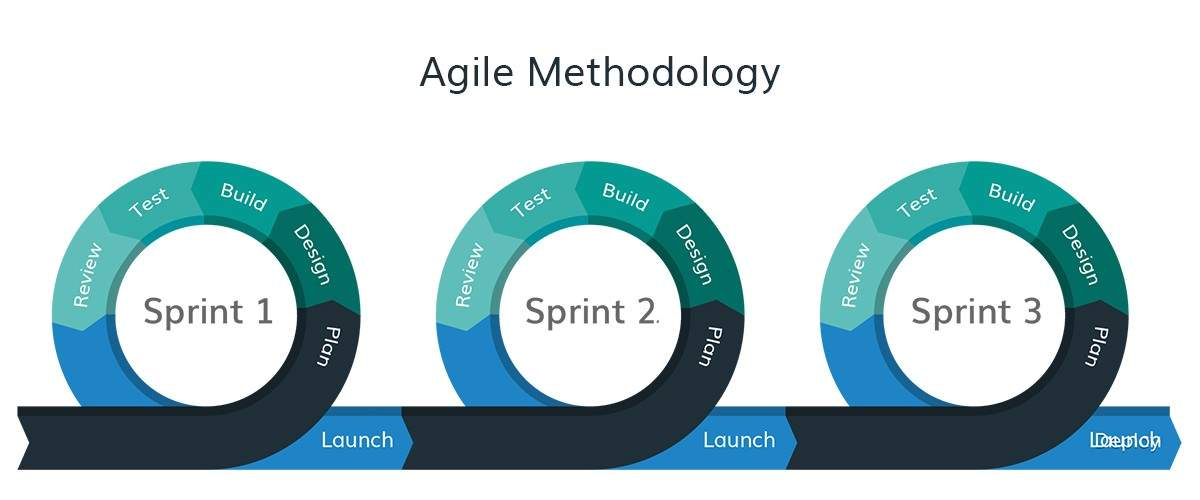
\includegraphics[width = 15cm]{agile_method.jpg}}
    \caption{Agile Scrum Methodology}
\end{figure}
Another advantage to using agile is that for the programming pattern that was used(see next section), the project can be broken down into features which then breaks down into entities and components(that do their own specific jobs) in a neat way, making it easier to create a feature early on, test it and then not have to refactor/touch it further into development as everything is highly decoupled. 

The project objectives as seen in the introduction are separated into two main sections (sprints), a \textit{Minimum Viable Product}, and then \textit{The Main Product}, which are broken down into multiple objectives, which act like their own sub-sprints going feature by feature).  

This methodology avoids having to do a big test of the program at the end of development as all the features are being tested rapidly while being created, so when the final prototype build was created, it works as expected.

\section{Programming Patterns}
The programming paradigm used was based around the Entity Component System (ECS) design where there are Entities in the world (the GameObjects) that are built up of components.

Games in Unity are built around this paradigm, preferring a system of composition over inheritance. It allows for greater flexibility as unlike inheritance where you 'inherit' all features at once, you build the game object using components(C\# classes) that you create that are designed to fulfill a very specific purpose. This leads to code being very modular and less coupled, leading to faster development and easier debugging as changing one component will not have a ripple effect on others, which is very much the case when designing a system around inheritance early on and then having to refactor it as you did not have enough foresight for a particular feature.
The following shows the flaws with inheritance for development\cite{CompOverInherit}:
\begin{lstlisting}
ROBOT // parent class
    .drive()
        MurderRobot // inherited class
            .kill()
        
        CleaningRobot // inherited class
            .clean()

ANIMAL // parent class
    .poop()
        Dog // inherited class
            .bark()

        Cat // inherited class
            .meow()
\end{lstlisting}
Now the above works great and would serve you through most of the project, but the problem arises if down the line you would like to create a \lstinline{MurderRobotDog} that can \lstinline{drive()}, \lstinline{kill()} and \lstinline{bark()}, however being a robot it cannot  \lstinline{poop()}. There are only a few solutions around this, 

1. you do a multiple inheritance and accept that you will have extra unnecessary functionality, 

2. you create a new Robot inherited from  \lstinline{MurderRobot} and duplicate the  \lstinline{bark()} functionality, 

3. you create a superclass of both that has a  \lstinline{bark()} functionality, this leads to unnecessary functionality in most instances. 

To solve this problem you will have to take time out from creating new features and refactor the codebase to work within good coding standards\cite{codingPractices}.

If designed using composition, it would look like the following (example from \cite{CompOverInherit}):
\begin{lstlisting}[frame=single]
ENTITIES          COMPONENTS (in the form of classes)
Dog             : pooper + barker
Cat             : pooper + meower
CleaningRobot   : driver + cleaner
MurderRobot     : driver + killer
MurderRobotDog  : driver + killer + barker
\end{lstlisting}
This provides you with the most flexibility to create whatever type of game object you would like while being loosely coupled and avoiding duplication.

Inheritance has its own benefits and was not abandoned, it was used in the places necessary, for example creating the \lstinline{BaseAIGoap} class.

In Unity, a game object with components attached to it can be saved as a prefab, which can then be reused, an example would be creating an enemy prefab, and then creating an enemy spawner that loads copies of that prefab into the scene.

\section{Tools}
%tools
% need to add
% - evaluation tool

\subsection{Unity (Game Engine)}
Unity\cite{unity} was chosen as the game engine, over the other options which was Unreal Engine\cite{unrealEngine}, as the author had some prior (albeit minimal) experience in using it; Unity used C\# for scripting which is a simpler language to write in over C++, with the drawback of providing fine-grain memory control (which was not required in this project). The Unity game engine also performs dramatically better on the hardware and operating system used to create this project.

Godot, an open-source game engine, was another option that could be used however it lacks in maturity for both documentation and feature set for 3D development\cite{godot}. As mentioned in the PDD, Unity has an extensive amount documentation available on their website which is easy to understand, they also have a forum site where there is a very active community in helping new-comers with any issues they face; as well as this, there are plenty of tutorials teaching Unity and its plentiful features on their own website and on YouTube.

There is also an asset store built into Unity with many paid and free assets, ranging from scripts, models, materials, shaders, physics systems and more.

All of this combined, it was very difficult for me to not choose Unity as the game engine of choice for my project.

\subsection{JetBrains Rider (IDE)}
JetBrains Rider was the choice of IDE as I had been using JetBrains products since the Programming in Java module in the first year. JetBrains provide a very good set of refactoring and debugging tools with a good amount of community made extensions for the program. Rider was created as a .NET IDE, and now has native Unity support, which is perfect for use with Unity.

My other option was Microsoft's Visual Studio, which I had used in the second and third year Games Tech modules. After using it extensively, it did not provide many of the features that I would expect from an IDE and had installed the plugin ReSharper created by JetBrains to bring some extra functionality required. Given that JetBrains have their own IDE for Unity, I decided to go with that over Visual Studio.

\subsection{GitHub}
GitHub was the choice of version control and backup system as I am very familiar with it. I have used it extensively over my time at the university.

One branch was used as this was not a large project and a commit was made at the end of a notable change. A full Git Log histr can be found in the appendices.

\subsection{Blender}
Blender was the 3D program of choice as it is very intuitive to learn and very simple to use. It is also free and open source leading to very many tutorials and big community around it along with great documentation. It has support for opening most 3D file-types which is very important as assets will be downloaded from different locations; if there is a filetype that is not supported, then there is bound to be an extension for it, due to the many community made extensions available.

\subsection{Adobe Illustrator}
Adobe Illustrator was the choice of vector editor used to design and plan any graphical elements in the game. 

\subsection{diagrams.net}
Diagrams.net (formally known as draw.io) was used as the tool to create UML diagrams as it is a lightweight web-application providing all the necessary features and flexibility required in creating a UML document. The feature that came in most useful was the integration with github; I was able to save my diagrams and version them directly in the same repository.

% \subsection{Plant UML}
% Plant UML is an open source UML creation tool allowing you to write UML in plain text. This was used to create a UML diagram out of the final code output.


\section{Software Design}

\subsection{Modelling Actions}
The actions for the AI agents were modelled before modelling the class diagrams. This was done so that the preconditions, effects and the goals they fulfil are mapped out and make it much easier to plan out the different classes.

\subsection{Class Diagrams}
Class diagrams are a great to draw out a visual plan of what the system will look like. As I am using an ECS form of design, the class diagram will mainly consist of many classes with compositional relationships. The class diagram contained a special shape that represents an action that were modelled prior to this. 
This class diagrams created are not a one-to-one representation of the code to be implemented, however a guideline to proceed with as there is a plan in mind before implementing it; while implementing, new and better ideas might arise that can and are used, this is only possible as there is structure to the development.

\subsection{User Interface (UI)}
Adobe Illustrator was used to draft out the user interface. Some UI elements will exist within the 3D world space, these are called \textit{spacial} UI elements; these types of UI elements allow the player to receive the information they require without taking up much space on the orthographic canvas where more player related statistics can go\cite{UIChoices}. These also help greatly during development to visualise the statistics without looking at the inspector in Unity.

\section{Project Objectives}
The project was created by going through the objectives stated in the introduction and tackling them one at a time, breaking each task down when arriving to it, this way there was focused attention on each feature being added in, being tested and refined before moving on to the next feature.

%=========================
%   Results
%=========================
\chapter{Result}

\textit{\textbf{Note:}} There are many code listings in this chapter, explaining some key aspects of the program, the comments on these are different to the ones in the actual code as to explain it thoroughly here, so keep in mind the explanation for methods is done in both \textit{comments and text}.

% Milestone 1
\section{Minimum Viable Product}
This section goes thoroughly through the steps taken and the output of those steps taken to achieve the objectives set out in the introduction.
\subsection{Modelling the Actions}
The AI system was abstracted into the different actions the AI will be performing and the goals it will use to plan out the course of action. Seen in the figure below is the simple set of actions and goals sufficient for the first build and will have the groundwork to expand upon the next build. The food ready goal and precondition for eat food will be used to add the attacks for the creature's higher in the food chain, like the Lizard, as they should only be able to eat other creatures if they are dead, i.e. ready to eat.

\begin{figure}[H]
    \centering
    \fbox{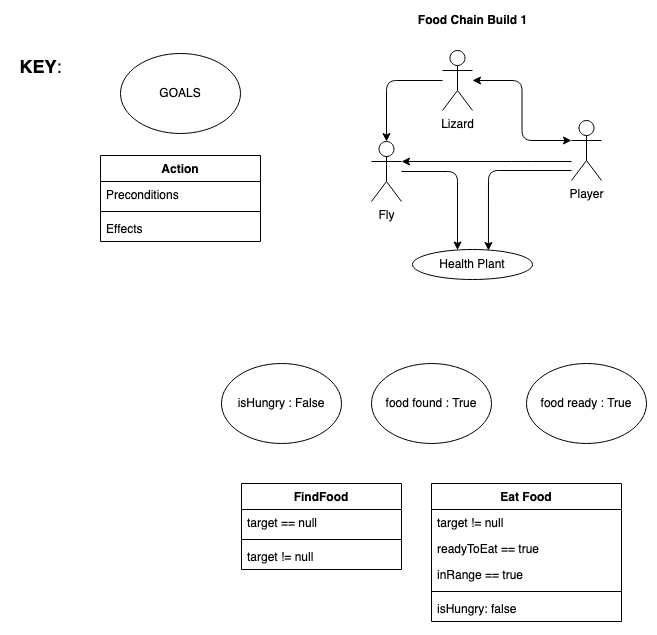
\includegraphics[width = 10cm ]{Actions and food chain build 1.png}}
    \caption{Goals and Actions with Food Chain}
\end{figure}

\subsection{Class Diagram}

\begin{figure}[H]
    \centering
    \fbox{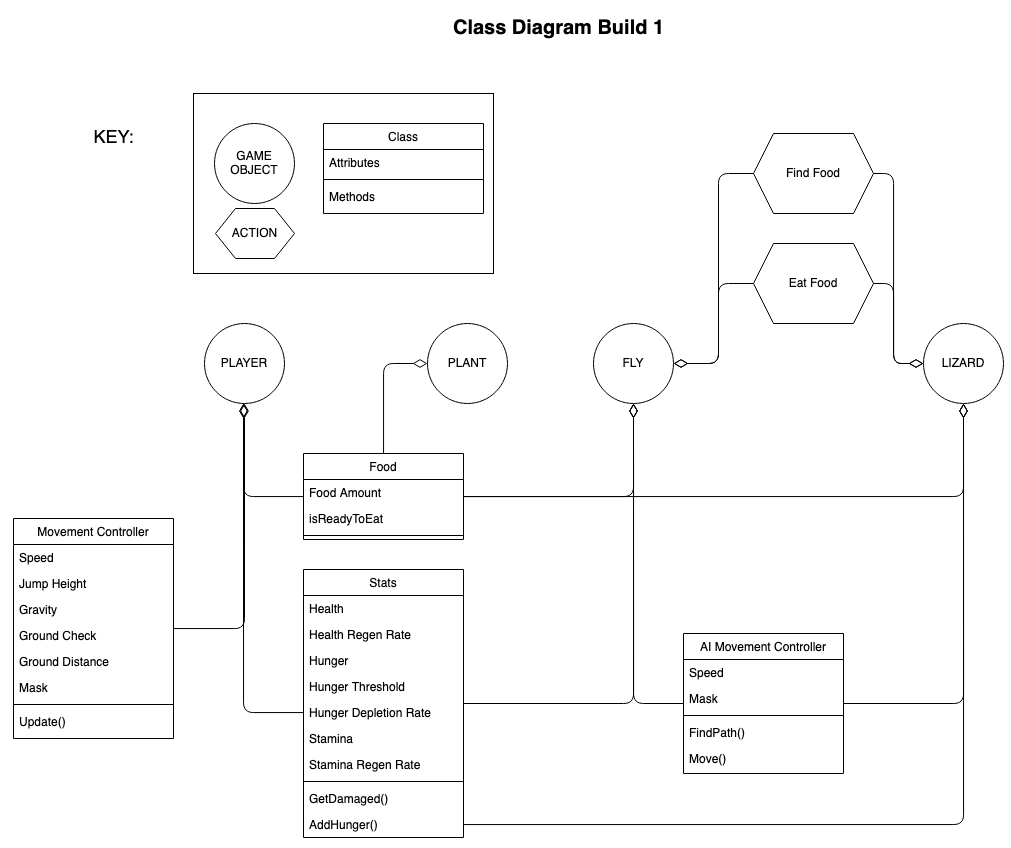
\includegraphics[width = 14.5cm ]{ClassDiagramBuild 1.png}}
    \caption{Class Diagram build 1}
\end{figure}

As explained before, Unity uses the Entity Component Paradigm of software design, the circles represent Game Objects which are the entities in our game scene, and there are classes attached to them using compositional relationships, as you can see, one class is being used multiple times, and due to the lack of inheritance, there is very little interdependency. 
The Actions are represented by hexagons are the actions modelled out in figure 6.1, it had been kept simple at this moment as it was not certain on what methods would be used to create the goal oriented action planning system.

\subsection{Creatures and AI}
Extensive reading through the FEAR SDK\cite{fearSDK}, that contains the full AI source code, was done to fully understand the implementation of GOAP.
Many other implementations of GOAP were also analysed and came to a conclusion that all of them are implemented in a very similar way with mostly only structural differences. 
Peter Klooster created a multi-threaded GOAP System for Unity3D which he originally used in his game Basher Beatdown \cite{basherGoap}. This is a pretty simple implementation that includes a visualiser for the system as well.
Anne from the YouTube channel TheHappieCat did a GOAP implementation in Unity \cite{happieGoapVideo} based on the papers by Jeff Orkin and an article by Brent Owens \cite{brentOwensGoap} (taking the core system from here). She made a very informative video on the topic as well as walking through the code with a live simple example.
On Jeff Orkin's website, there was a reference to ReGOAP by Luciano Ferraro, which is a very generic C\# GOAP library, that was used in Unity3D, but its description states it can be used anywhere. Compared to the other implementations, this has been officially released on the Unity Asset store, however the code seems to be quite verbose and is not well commented and documented.

Based on this research, the author started creating a GOAP system from scratch, however, it became very time-consuming to create, and based on the gannt chart created, the project was running behind on schedule; as the main focus of the project is to create the interaction between these different AI agents, and not the core AI system itself.

The author then looked through the different GOAP implementations stated and their example projects and tried to create a simple agent with all three systems, after that, a conclusion was drawn to utilise the implementation provided by Brent Owens \cite{brentOwensGoapCode} which is under the MIT licence. This is a very bare bones implementation only consisting of 6 scripts, and with the video explanation by TheHappieCat this proved to be the simplest one to implement and still have a great amount of flexibility in modifying the code due to its small size in number of scripts.

% After landing on this implementation of GOAP, the different actions were modelled (with their preconditions and effects (post-conditions)), with the different creatures with their world state and the list of goals they would like to achieve. 

To add GOAP AI behaviour to an Agent, a script had to be attached that implemented the \lstinline{IGoap} interface provided by Brent Owens, and then have the \lstinline{GoapAgent} script attached which uses the \lstinline{GoapPlanner}. Now actions (inherited from \lstinline{GoapAction}) can be attached as scripts to the game object and the planner will automatically consider them. The script that inherits \lstinline{IGoap} will contain the world state and the desired goal state. The \lstinline{GoapAction} s will contain their own \textbf{preconditions} and \textbf{effects} and a \textbf{procedural precondition} method that the planner will consider when choosing the plan of action. 

\begin{lstlisting}[language=c]
// inside Creatures : IGoap 
// world state
worldData.Add(new KeyValuePair<string, object>("isHungry", (hunger < hungerThreshold)));
// goal
goal.Add(new KeyValuePair<string, object>("isHungry", false));

// For Lizard that inherits creature
worldData.Add(new KeyValuePair<string, object>("damagePlayer", false)); 
goal.Add(new KeyValuePair<string, object>("damagePlayer", true));
 
// inside ActionEatFood.cs
addPrecondition("isHungry", true);
addEffect("isHungry", false);
cost = 1f;
\end{lstlisting}

This build of the AI was functional however had a few issues. The Lizard enemy would only choose the player and not the fly, and it would eat anything. A food chain was added in the main build to fix this.

As can be seen in figure 6.11 showing the UI for creature, the meshes for the creatures were kept simple to ensure that the AI system worked, the movement system was also a trivial direct vector transformation towards the direction of the target for the same reason.

\subsection{Player}
% Player movement
\subsubsection{Movement Controller}
The movement controller was implemented with the help from a tutorial by Brakey's on "First Person Movement in Unity - FPS Controller"\cite{fpsController}. To create this, a Player Empty was created, and a Mesh was added to it, in this case, a simple capsule was used; another empty was created that contained a Sphere Collider which checks collision with the ground to notify the Player Movement script that the player is grounded. The Player Movement script takes the Input from Unity's built-in input system and calculates the horizontal and vertical movement and then the script passes the movement data to the Character Controller to move the player. To jump, a check is made to see whether the player is grounded or not, and if so, then check for the Jump button to be pressed down, in this case, it is "Space"; a velocity is applied to the negative of the gravitational velocity and the player is jumping and no longer grounded. When the player is no longer grounded, a gravitational velocity is applied to the player constantly down.

% camera look
Now that the player was moving, the main camera had to be placed inside it, along with accepting mouse input to rotate the player and camera. Firstly the cursor is locked into the screen so when moving it, it does not leave the screen; then on every frame, the Mouse X and Y input is taken in, multiplied by the sensitivity and delta time. A rotation value is calculated, and is \textit{clamped} (minimum -90$^{\circ}$ and maximum 90$^{\circ}$); this rotation is then applied to both the local rotation of the camera, and the player's body rotation around it's up vector.
\begin{figure}[H]
    \begin{minipage}{.5\textwidth}
        \centering
        \fbox{\includegraphics[width = 5cm ]{{Player_Inspector_Character_Controller.png}}}
        \caption{Character Controller and Player Movement Scrpit components on the player}
    \end{minipage}
    \begin{minipage}{.5\textwidth}
        \centering
        \fbox{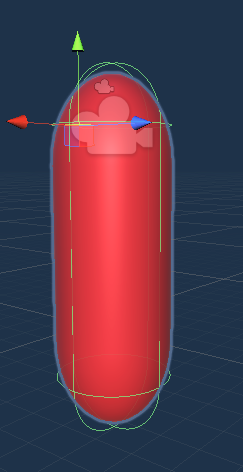
\includegraphics[width = 5cm ]{Player_Capsule.png}}
        \caption{The Player with the character controller bounding box and camera}
    \end{minipage}
\end{figure}

\subsubsection{Weapon}
For the melee weapon for the player to attack with, a pre-made sword asset was used (please refer to the asset listing) which was then imported into blender and 4 animation states were created. 

First the model was rigged using one bone, starting from the hilt of the sword. Then 4 different animations were created using key-framing and Blender's Dope Sheet editor, the idle animation and Attack 1 lasted 30 frames each and the Attack 2 and 3 lasted 20 frames each. This was then exported as an FBX file, which supports animations and textures to be baked into it and imported into Unity.
\begin{figure}[H]
    \begin{minipage}{.2\textwidth}
        \centering
        \fbox{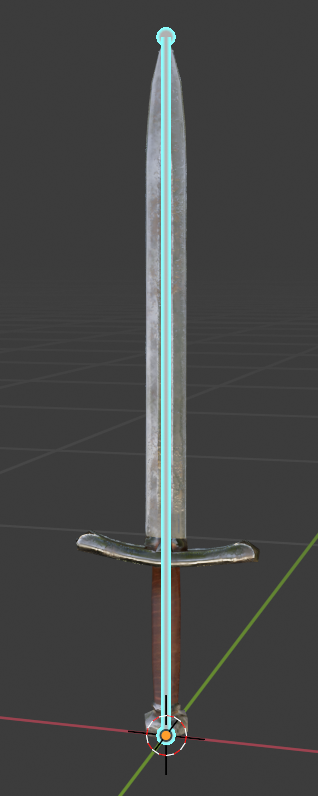
\includegraphics[width = 2cm ]{SwordBone.png}}
        \caption{Sword model rigged with a single bone}
    \end{minipage}
    \begin{minipage}{.8\textwidth}
        \centering
        \fbox{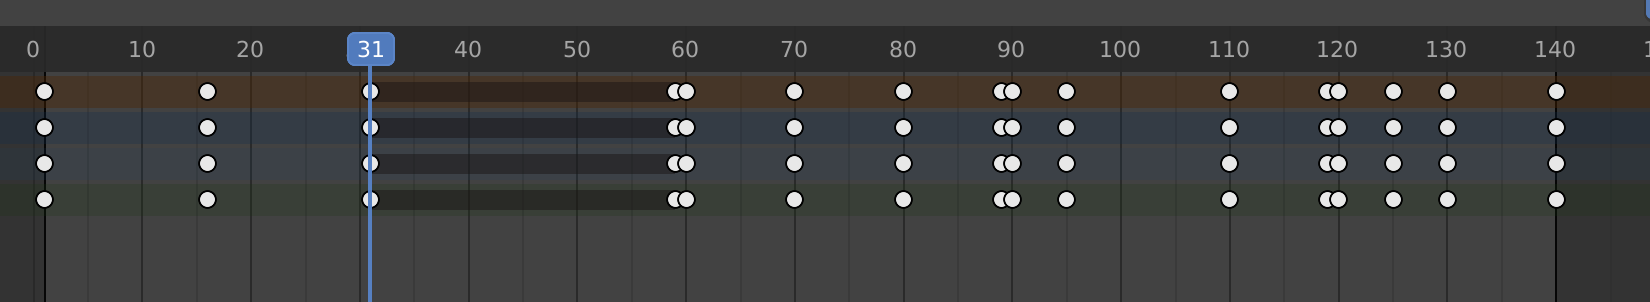
\includegraphics[width = 10cm ]{SwordKeyframes.png}}
        \caption{Dope sheet/Key-frames for 4 animations in Blender}
    \end{minipage}
\end{figure}

When importing it into Unity, the animations had to be split up into to 4 different actions as currently they were all done on one track (this was taken note of and the animations for the creatures were created on different tracks withing Blender, allowing an easier import process). In the heirarchy the sword was attached to an Empty called LeftHand to place it in the correct position, and this was parented under the Main Camera, making it so that the sword's transformation follows where the player is looking.

\begin{figure}[H]
    \begin{minipage}{.5\textwidth}
        \centering
        \fbox{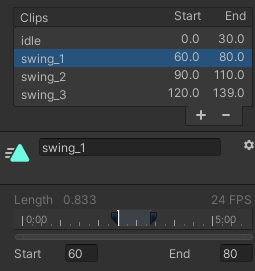
\includegraphics[width = 5cm ]{Sword_Unity_Animation_Import_Split.png}}
        \caption{Splitting Animations up for the Sword}
    \end{minipage}
    \begin{minipage}{.5\textwidth}
        \centering
        \fbox{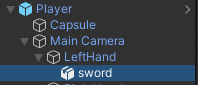
\includegraphics[width = 5cm ]{Sword_Unity_Heirarchy.png}}
        \caption{Sword in the Unity Hierarchy view}
    \end{minipage}
\end{figure}

An animation controller had to be created to switch between the different animations and create a combo system so a single click will only lead to the first swing, however clicking more than once will add the clicks to a buffer then swing the sword the appropriate number of times.

A tutorial by GRIMOIRE \cite{comboSystem} was used to understand how to do this inside of Unity and its animation system and implemented it in a similar manner.

\begin{figure}[H]
    \centering
    \fbox{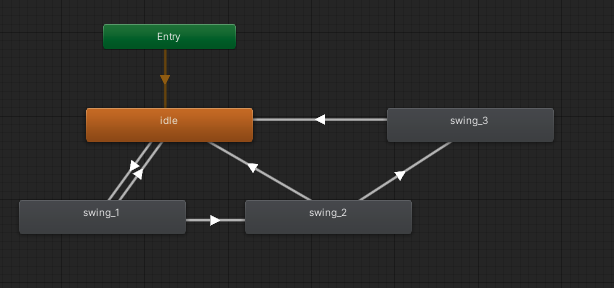
\includegraphics[width = 10cm ]{Sword_Animator.png}}
    \caption{Animation Controller attached to the Sword}
\end{figure}


\subsection{UI}
For the UI of the game, a decision was made to go without a main menu screen as there is only one level showcasing the use of the AI. 

The first UI designed was for the Creature displaying the stats above their meshes in game. This is one of the spacial UI elements in the game. Below is the initial sketch created in Adobe Illustrator.

\begin{figure}[H]
    \centering
    \fbox{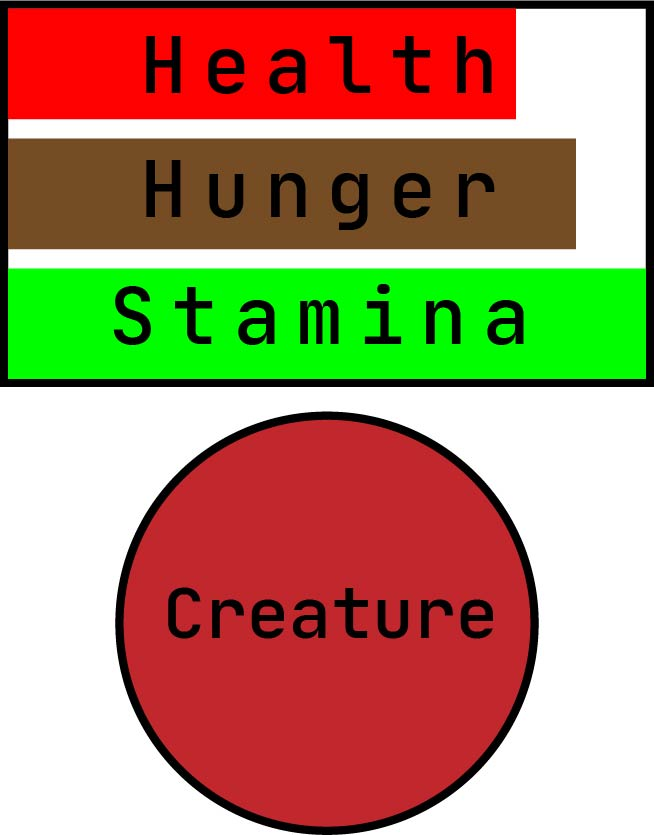
\includegraphics[width = 7cm ]{Stats_UI.jpg}}
    \caption{Creature UI Sketch}
\end{figure}

In Unity this was done by creating a canvas with multiple image sprites, these image sprites have a fill amount that goes from 0 to 1 which can be easily interpolated between by dividing the current values of the stat by their max value.

\begin{figure}[H]
    \begin{minipage}{.5\textwidth}
        \centering
        \fbox{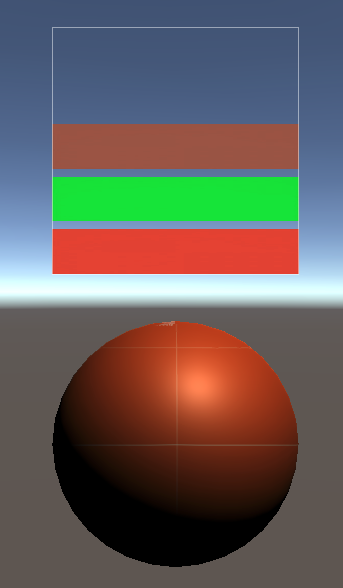
\includegraphics[width = 5cm ]{Stats_UI_Build1.png}}
        \caption{Creature UI in Unity}
    \end{minipage}
    \begin{minipage}{.5\textwidth}
        \centering
        \fbox{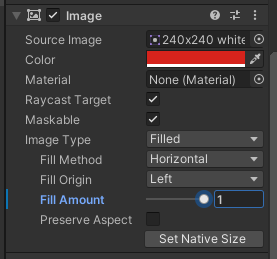
\includegraphics[width = 5cm ]{Unity_Image_Panel.png}}
        \caption{Image Component in Unity}
    \end{minipage}
\end{figure}

This canvas is parented to the Creature and the position is offset on the Y axis, so its transformation will follow its parent.

A script was created to manage the fill amounts, this was done by accessing a reference to the stats component in the parent object and then calculating the fill amount from there (see code snippet below).

\begin{lstlisting}[language=c]
void FixedUpdate() {
        healthBar.fillAmount = creatureStats.GetHealth() / 100;
        staminaBar.fillAmount = creatureStats.GetStamina() / 100;
        hungerBar.fillAmount = creatureStats.GetHunger() / 100;
        hungerThresholdBar.fillAmount = creatureStats.GetHungerThreshold() / 100;
}
\end{lstlisting}

\subsection{Unity Project}

Below is what the first version of the Unity scene looked like after adding the sword and basic AI components in. A very basic level was created to test out the movement controller for the player, along with physics interaction of the sword. The materials applied are a mix of simple self-made materials from the Unity asset store called "Gridbox prototype materials by Ciathyza", (see asset listing).

\begin{figure}[H]
    \centering
    \fbox{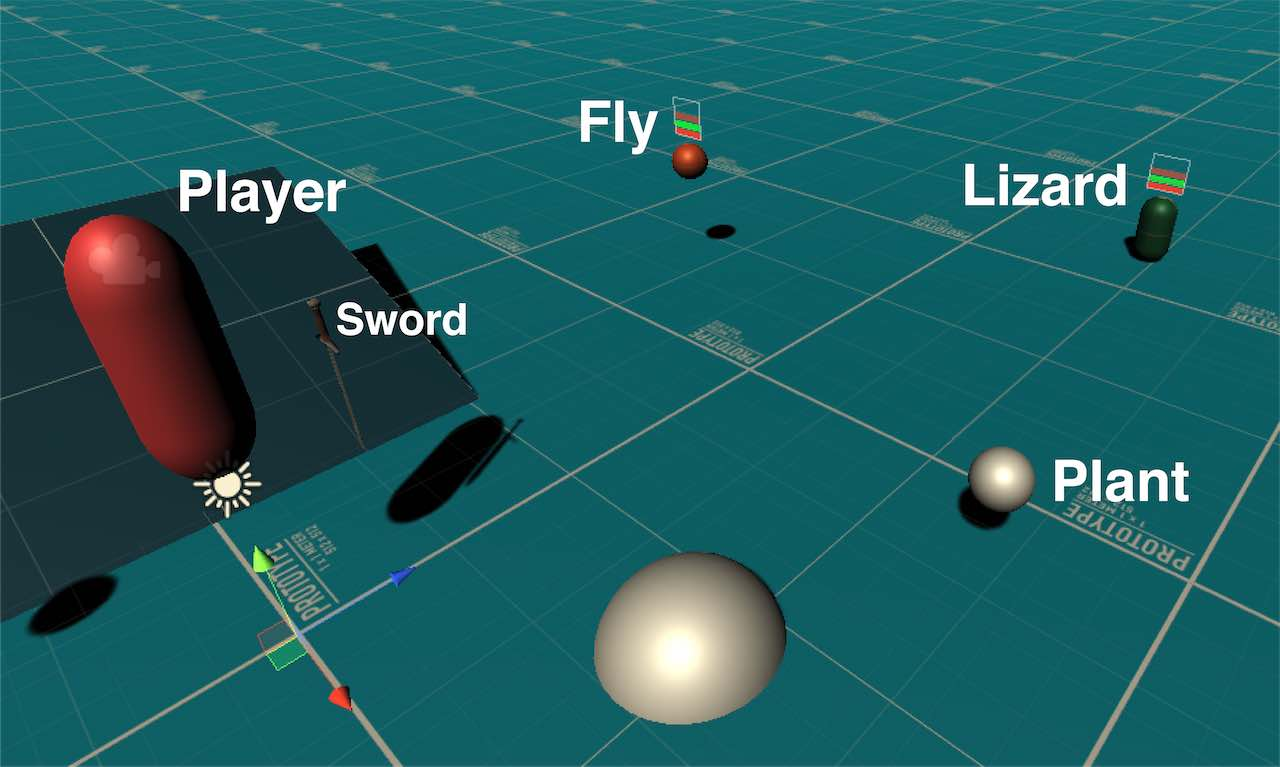
\includegraphics[width = 15cm]{Unity_Scene_Build_1_annotated.jpg}}
    \caption{Annotated view of Unity Scene}
\end{figure}



\section{Main Product}
\subsection{Creatures and AI}
\subsubsection{Meshes}
The meshes of the creatures were changed; a set of animated ice age animal meshes by Riley on itch.io (please see in the asset listing). These were aesthetically pleasing while having a low poly count keeping the file size and performance overhead to a minimum. 

The saber-tooth (replacing the lizard in the food chain) had 4 animation states, of which only 3 were required, however the sloth (replacing the fly in the food chain) only had 2 animation states, walk and idle, an additional one for biting was required for when it eats food. 

The model was imported into Blender, however the model seemed to have an unnecessary number of bones, most of which did not have an effect to the model. Seeing this, the model had to be rigged again and freshly animated. The same process was used as the sword but with a higher complexity.



\begin{figure}[H]
    \begin{minipage}{.5\textwidth}
        \centering
        \fbox{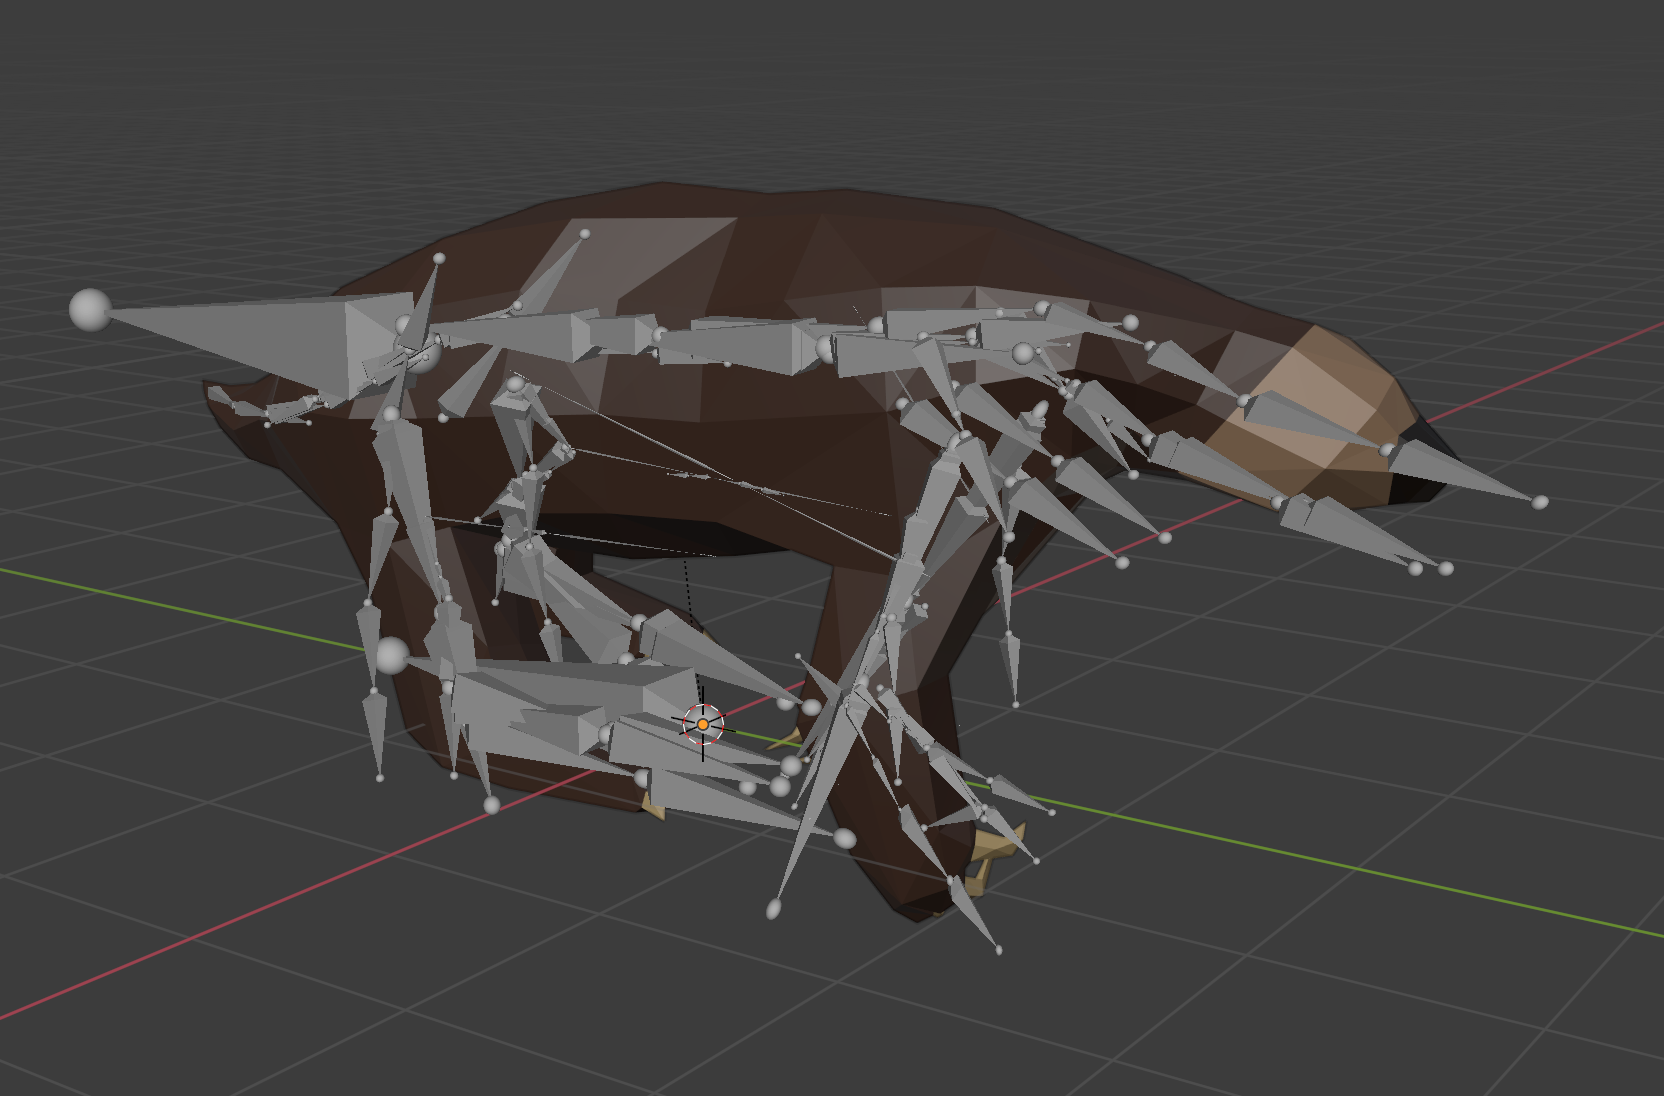
\includegraphics[width = 7cm ]{Sloth_Model_Messy_Rig.png}}
        \caption{Messy Original Sloth Rig}
    \end{minipage}
    \begin{minipage}{.5\textwidth}
        \centering
        \fbox{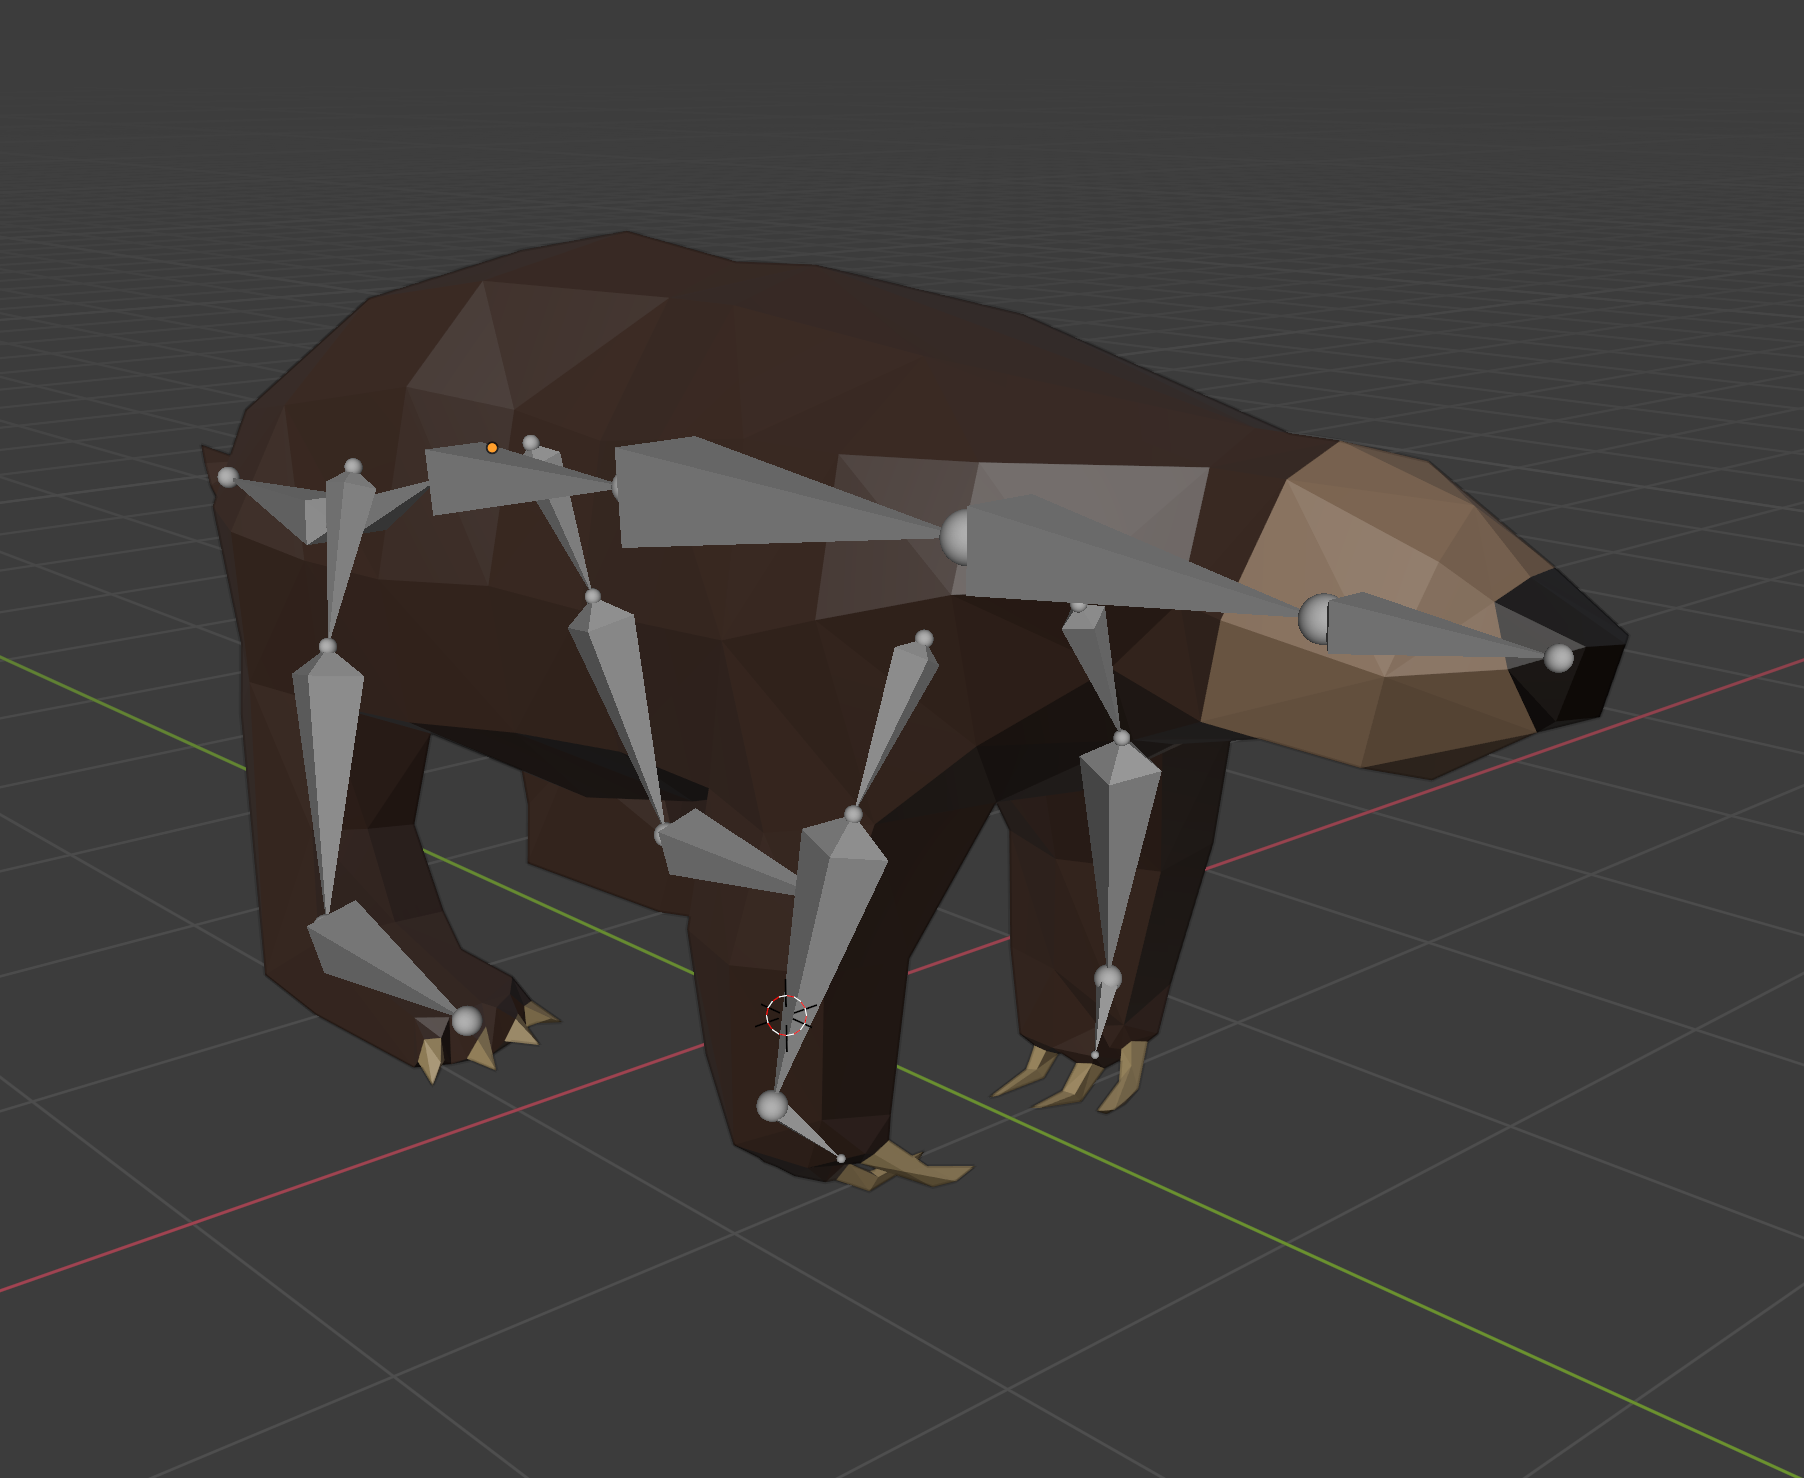
\includegraphics[width = 7cm ]{Sloth_Model_Clean_Rig.png}}
        \caption{Clean New Sloth Rig}
    \end{minipage}
\end{figure}


\subsubsection{Class Diagram Updated}

The class diagram was updated to add in the Attacks for the lizard enemy, the A star game object for the pathfinding and the food chain game object.

\begin{figure}[H]
    \centering
    \fbox{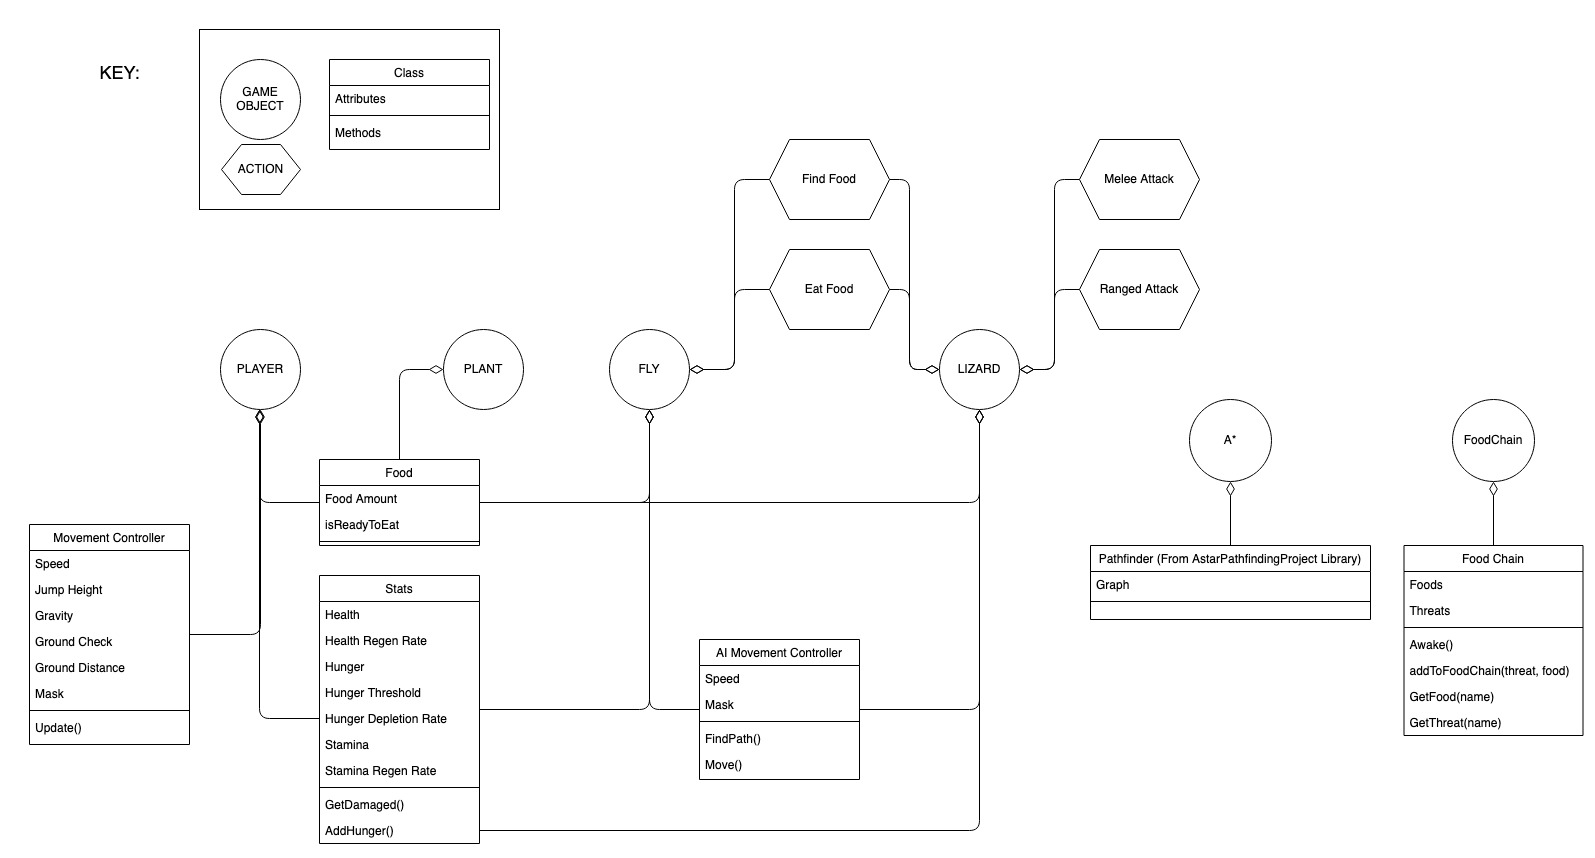
\includegraphics[width = 15cm]{ClassDiagram.jpg}}
    \caption{Updated Class Diagram}
\end{figure}

% Food Chain
The Food Chain game object is unique in that there is only one required in a scene, and the Find Food action will access it to find out what the state of the food chain is to find food that is appropriate to that creature. Below is the code that is attached to the food chain game object.

On load, it will create a food chain based on the relationships we provide there. There are constant string references to access the names of the creatures in the food chain at any point.

Any game object in the scene can access this food chain and call GetFood(their name) and get the foods that they can eat, and vice versa with what they consider threats. \footnote{This was created without the knowledge of Bi-Directional Dictionaries (however is structured similar to one and one might work better), during the final days of this project, an article was found which explains how to create a bi-directional dictionaries using an interface \cite{biDirectionalDictionaries}.}

\begin{lstlisting}[language=c]
// FoodChain.cs : has been abridged to show in report
    // predators
    private Dictionary<String, HashSet<String>> threats = new Dictionary<string, HashSet<string>>();
    // preys
    private Dictionary<String, HashSet<String>> foods = new Dictionary<string, HashSet<string>>();
    // in the awake method create the food Chain
    private void Awake() {
        // Create the food chain
        addToChain("player", "sabertooth");
        addToChain("player", "sloth");
        addToChain("player", "plant");
        addToChain("sabertooth", "player");
        addToChain("sabertooth", "sabertooth");
        addToChain("sabertooth", "sloth");
        addToChain("sloth", "plant");
    }
    private void addToChain(String threat, String food) {
        //add to foods list
        if (foods.ContainsKey(threat)) 
            foods[threat].Add(food);
        else 
            foods.Add(threat, new HashSet<string>() {food});
        // add to threats list
        if (threats.ContainsKey(food)) 
            threats[food].Add(threat);
        else
            threats.Add(food, new HashSet<string>() {threat});
    }
    // Get the the Set of foods for the given creature
    public HashSet<String> GetFood(String name) {return foods[name];}
    // Get the the Set of threats for the given creature
    public HashSet<String> GetThreat(String name) {return threats[name];}
\end{lstlisting}


\subsubsection{Pathfinding}
A path finding system was added (as seen in the updated class diagram) in to facilitate better movement for the AI Agents. A* Pathfinding Project by Aron Granberg (see asset listings). This is a very nice and free library that provides the generation of many type of nav meshes, the one used in the game is a Grid Graph, which is the 'most straight forward path' and can be updated during runtime if obstacles move, it is not the most performance efficient type of graph as all the nodes in the grid are equidistant from each other, and in a large open space, that amount of detail/resolution in the grid is not required; however for our purposes, this type of graph is more than capable. 
\cite{astarPathfinding}
\begin{figure}[H]
    \begin{minipage}{.5\textwidth}
        \centering
        \fbox{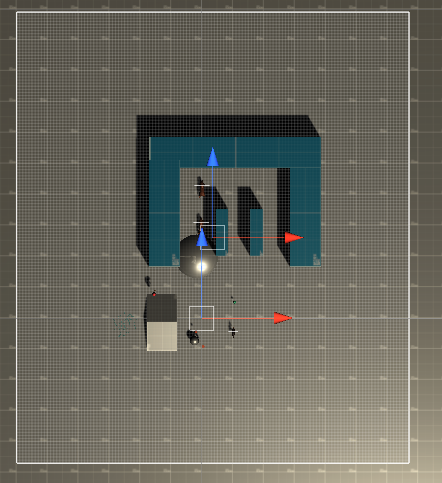
\includegraphics[width = 7cm ]{AStar_Graph.png}}
        \caption{A-Star Grid Graph in scene}
    \end{minipage}
    \begin{minipage}{.5\textwidth}
        \centering
        \fbox{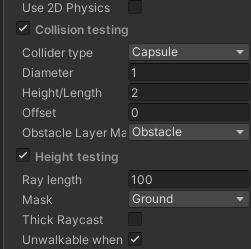
\includegraphics[width = 7cm ]{AStar_CollisionSettings.png}}
        \caption{Settings for collision testing}
    \end{minipage}
\end{figure}

In figure left you can see the graph being scaled appropriatly for the level, and in figure right are the settings for collision testing and removing obstacles as walkable in the nav-graph. Unity provides the ability to assign a layer to game objects. In this case, a layer called \textbf{Obstacle} has been applied to the blue boxes seen, so this gets masked out of the scan. As seen in height testing, The \textbf{Ground} layer (applied to all grey objects in scene) has been added as the mask to test the height, this avoids any chance of having a floating graph.

\begin{figure}[H]
    \centering
    \fbox{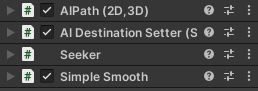
\includegraphics[width = 7cm]{Astar_AgentComponents.png}}
    \caption{Components for Agents to use A Star Pathfinding}
\end{figure}

Now for the agents to use this graph, a few components provided by the library were attached. As seen in the figure above. The \textbf{AIPath} contains the movement controller for the agent to move along the discovered path and contains the shape(radius and height) of the agent, to ensure it does not go into the obstacles. The \textbf{AI Destination Setter} component contains a \textbf{Target} transform property, this is the transform the seeker will use to find a path. The \textbf{Seeker} component references the target and the A* Graph to find a possible path, which the AIPath component will use. \textbf{Simple Smooth} is an optional component that takes the path produced by seeker and smoothen it out.


\subsubsection{Goap AI}
% New Actions
The AI system was expanded upon in this build. The action for \textbf{Find Food} was refactored to make use of the newly created food chain; changes were also made so that there was a vision cone to what a creature can detect, this is 90$^{\circ}$ straight in front of the head as seen in the figure below.
\begin{figure}[H]
    \centering
    \fbox{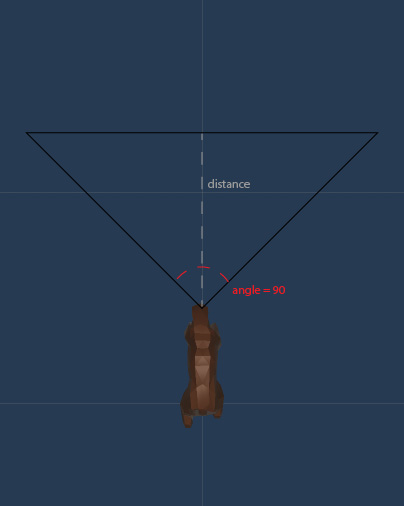
\includegraphics[width = 7cm]{Vision_Cone_Representation.jpg}}
    \caption{Vision Cone Represented}
\end{figure}

The \textbf{Eat Food} action can only be executed now if the food is ready, and to make the food ready, it needs to be killed, and therefore the planner will find and execute the \textbf{Melee Attack}.

Both these actions were also changed to play the animations at the correct moment.
The Creature class from build one was broken down into an abstract BaseAIGoap class that inherited the IGoap interface and provided implementation for the methods that log on action complete/fail/etc.; a boolean check was created so that the programmer can disable the logging to the console, as this has a major hit on performance in Unity and also cluttered up the console when multiple agents were active, essentially making it unusable. The \textbf{Sabertooth} and \textbf{Sloth} now inherited from this and applied their goal states seperatly, reducing the coupling and making debugging simpler than when they inherited from a Creature class.
\begin{lstlisting}[language=c]
// This class inherits IGOAP to provide implementation for methods on finishing the plans.
public abstract class BaseAIGoap : MonoBehaviour, IGoap {
    // if this is true then print output to console
    public bool enableDebugging = true;
    // world state of the agent will be inherited
    public abstract HashSet<KeyValuePair<string, object>> getWorldState(); 
    // desired goal state of the agent will be inherited
    public abstract HashSet<KeyValuePair<string, object>> createGoalState();
    // implement this method by having a check to print the output or not
    public void planFound(HashSet<KeyValuePair<string, object>> goal, Queue<GoapAction> actions) {
        // found a plan for our goal
        if(enableDebugging)
            Debug.Log(gameObject.name + ": <color=green>Plan found</color> " + GoapAgent.prettyPrint(actions));
    }
    // similar thing applied to following methods
    public void actionsFinished() {...}
    public void planAborted(GoapAction aborter) {...}

    // Move agent exists in IGOAP to move to the object to perform the action
    public abstract bool moveAgent(GoapAction nextAction);
    // this is a method I created which will be different for different agents, it performs all the things to start and stop moving the agent.
    public abstract void StartMoving(bool toMove, Transform target);
}
\end{lstlisting}


% Problem with no partial plan of action
After the adding the pathfinding and the new actions into the game, the agents behaved as expected until \textit{\textbf{they had not found a target and were hungry}}. In this case, the agent would just be in an idle state and not do anything, where it was expected to perform \textbf{Find Food} and then \textbf{Eat Food}. This was occurring because as the current planning system did not accept partially successful plans (a series of actions that do not fulfill \textbf{every} goal state), which was quite unusual as there are many cases where some actions/series of actions do not tick every box, and the correct behaviour in this scenario would be to perform a partial plan if a full plan is not found.

In this particular case, the problem was that \textbf{Find Food} did not directly have an effect of \textbf{isHungry == null}. This could be mitigated by adding that as an effect of \textbf{Find Food}, however this would be lying and would incur in complications and tight coupling further down the line when creating a more complex AI system, where one of the main advantages of GOAP is that it provides a modular, loosely coupled approach to AI.

There were many solutions that came to mind, however most of these lead to heavy refactoring of the AI code, and this was not feasible this late in the development of this project as it would have put a stop on an already tight schedule.

% First use of the AUTHOR ?????
So the solution that the author went with provided the most minimal amount of refactoring and still provided desirable results in most use cases.

In the \textbf{Goap Planner} script, there is a method that is called recursively called \lstinline{buildGraph()}, which goes through all possible actions and creates a graph of possible plans, it checks if the plan is fully successful by using the \lstinline{inState()} function; it then compares the \textit{costs} of these plans and picks the lowest cost one.

Based on the above observation, \lstinline{inState()}  had to be somehow changed to let \lstinline{buildGraph()} know there was a partial match and do something with it. So now \lstinline{inState()} takes in a boolean by reference called \lstinline{partial} which is set to true if a partial match is found; and in build graph this is only checked if a full solution was not found.

\begin{lstlisting}[language=c]
// GoapPlanner.cs
// buildGraph()
......
Node node = new Node(parent, parent.runningCost + action.cost, currentState, action);
partial = false;
// partial gets assigned a value in this call to inState
if (inState(goal, currentState, ref partial)) {
    // a solution is found   
    ...
}
// if it is a partial match, then It will scale the cost by 10
else if (partial) {
    // we found a partial solution
    // scale the running cost if it is a partial match, therefore prioritising full matches
    node.runningCost *= 10; 
    leaves.Add(node);
    foundOne = true;
}
else {
    // not at a solution yet, so recursivley test all the remaining actions and branch out the tree
    ...
}
......

/**
* Check that all items in 'test' are in 'state'. If just one does not
* match or is not there then this returns false. If it is a partial
* match however, the parameter passed through by reference 'partial'
* will be set to true.
*/
private bool inState(HashSet<KeyValuePair<string, object>> test, HashSet<KeyValuePair<string, object>> state, ref bool partialMatch) {
   bool allMatch = true;
   foreach (KeyValuePair<string, object> t in test) {
       bool match = false;
       foreach (KeyValuePair<string, object> s in state) {
           if (s.Equals(t)) {
               match = true;
               // if there is a single match, partial match will be set to true
               partialMatch = true;
               break;
           }
       }
       if (!match)
           allMatch = false;
   }
   return allMatch;
}



\end{lstlisting}

\subsubsection{Ragdolls}
When destroyed, there was no state for the creatures to be in, so it was decided that ragdolls would be fun to allow the player to move the body around using the physics based collisions on the sword and the crossbow weapons, and it would also provide a clear indicator that the creature is dead.

Unity has a built-in Ragdoll creator, however that only works on humanoids with the appropriate bone structure (for the armatures), so it had to be done manually for each creature. A YouTube tutorial was used to understand what components were required on what to achieve this effect. \cite{RagdollTutorial}
\begin{figure}[H]
    \begin{minipage}{.5\textwidth}
        \centering
        \fbox{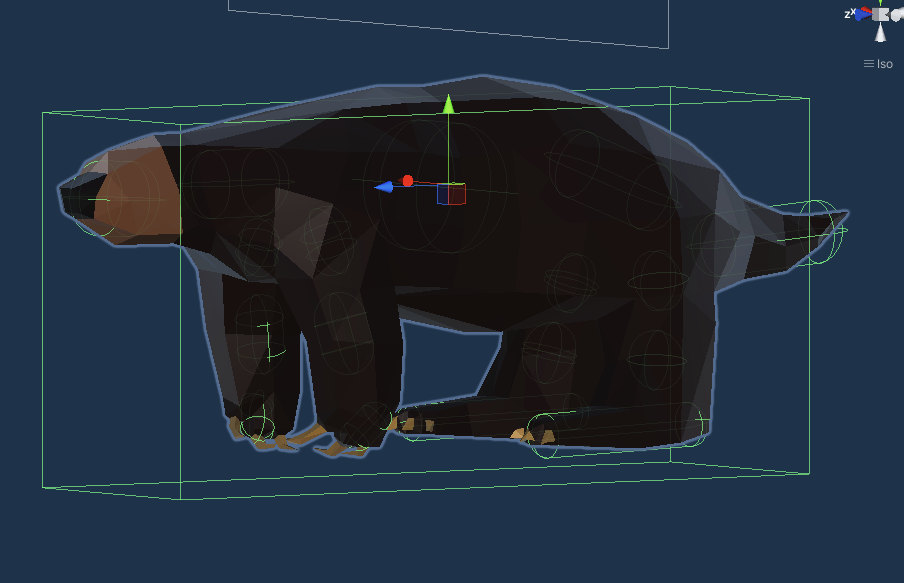
\includegraphics[width = 7cm ]{Ragdoll_Colliders.png}}
        \caption{Colliders on the Creature in Green}
    \end{minipage}
    \begin{minipage}{.5\textwidth}
        \centering
        \fbox{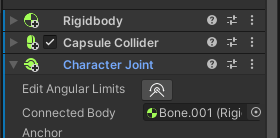
\includegraphics[width = 7cm ]{Ragdoll_Inspector.png}}
        \caption{Rigidbody, Collider and Character Joint applied to bones in the armature.}
    \end{minipage}
\end{figure}
There are two groups of colliders applied to the creatures, one is a box collider which is active when the creature is alive, allows simple physics interaction and the player's weapons; the second group are the capsule colliders applied to the necessary joints in the character, a character joint needs to be applied to every child node to tell Unity what bone it is attached to. Both these groups cannot be activated at the same time as overlapping colliders causes rigidbody physics to misbehave.

A Ragdoll Toggle script was created which enables and disables the appropriate colliders.

\begin{lstlisting}[language=c]
// storing the colliders when the game object is loaded
private void Start(){
    boxCollider = GetComponent<BoxCollider>();
    childrenColliders = GetComponentsInChildren<Collider>();
    childrenRigidbodies = GetComponentsInChildren<Rigidbody>();
}

// method that and enables/disables appropriate colliders
public void EnableRagdoll(bool isActive) {
    // children colliders
    foreach (var collider in childrenColliders) {
        collider.enabled = isActive;
    }
    // children rigidbody
    foreach (var rigidbody in childrenRigidbodies) {
        rigidbody.detectCollisions = isActive;
        rigidbody.isKinematic = !isActive;
    }
    // parent
    animator.enabled = !isActive;
    boxCollider.enabled = !isActive;
    aiComponent.enabled = !isActive;
}

// this is later called in Stats.cs when a creature dies
private void Death() {
    if (isThereRagdoll) {
        ragdoll.EnableRagdoll(true);
    }
}
\end{lstlisting}

\subsubsection{Particle Effects}
On applying damage via the Stats component, blood particles are spawned, and these blood particles are specified per creature, allowing for different particle effects per enemy type. 

\begin{figure}[H]
    \begin{minipage}{.5\textwidth}
        \centering
        \fbox{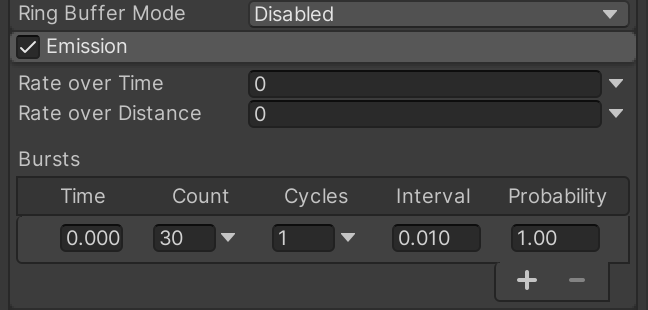
\includegraphics[width = 7cm ]{Particles_Burst_Emmision.png}}
        \caption{Burst Emmision of Particles}
    \end{minipage}
    \begin{minipage}{.5\textwidth}
        \centering
        \fbox{
\includegraphics[width = 7cm ]{Particles_Destroy_OnStop.png}}
        \caption{Destroy Instance on stop}
    \end{minipage}
\end{figure}

For now there one set of blood particles for all enemies. They are set to do a single burst of 30 particles at the beginning, and reduce their size over their lifetime to 0, and when the particle has finished, it will destroy itself. 

% EAT PARTICLE EFFECTS
A similar system was created when a creature or the player eat another creature. Two different materials were created for this, brown particles for eating a flesh based enemy, and green particles for plant based foods, these can be applied per creature, so it is very flexible to replace particles for different enemies.

\begin{figure}[H]
    \begin{minipage}{.5\textwidth}
        \centering
        \fbox{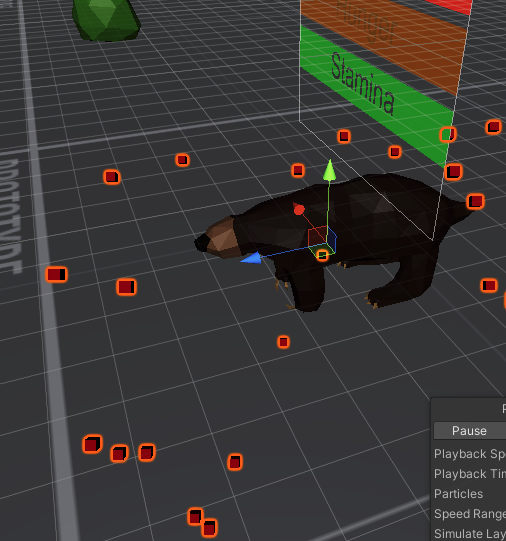
\includegraphics[width = 7cm ]{Particles_Blood.png}}
        \caption{Blood Particles}
    \end{minipage}
    \begin{minipage}{.5\textwidth}
        \centering
        \fbox{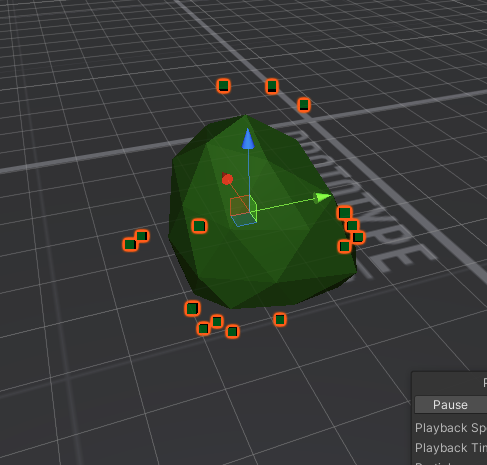
\includegraphics[width = 7cm ]{Particles_Plant_Food.png}}
        \caption{Food Particles for Plant}
    \end{minipage}
\end{figure}

\subsection{Player}
% TODO EAT
\subsubsection{Eating}
The ability to eat other creatures was added. This was done by sending a thick ray cast (Sphere Cast in Unity) from the center of the camera's view point to check for any collisions, if this ray cast collides with an entity within the 'Life' layer, and it is ready to eat, the player will be able to press 'E' to eat the food. A HUD element was created to represent the player's ability to interact with the creatures.
\begin{lstlisting}[language=c]
...
RaycastHit hit; // the point of contact
if (Physics.SphereCast(origin, thickness, direction, out hit, maxDistance, lifeLayerMask)) {
    ...
    if (hit.transform.root.GetComponent<FoodStats>().isReadyToEat) {
        if (Input.GetKeyDown(KeyCode.E)) { // press E
            stats.AddFoodAmount(hit.transform.root.GetComponent<FoodStats>().foodAmount); // add food
            hit.transform.root.GetComponent<FoodStats>().DepleteTotalFoodAmount(hit.transform.position, hit.transform.rotation); // deplete from prey and spawn particles
        }
    }
    ...
}
...
\end{lstlisting}

\subsubsection{Weapons}
% Sword
Two colliders were attached to the sword, a box collider to interact with other physics objects; and a mesh collider that conforms around the sword, which behaves as a trigger with no physics interaction. In Unity, when a "GameObject collides with another GameObject, it calls \textbf{OnTriggerEnter}" \cite{UnityTriggerCollider}.  
\begin{figure}[H]
    \begin{minipage}{.3\textwidth}
        \centering
        \fbox{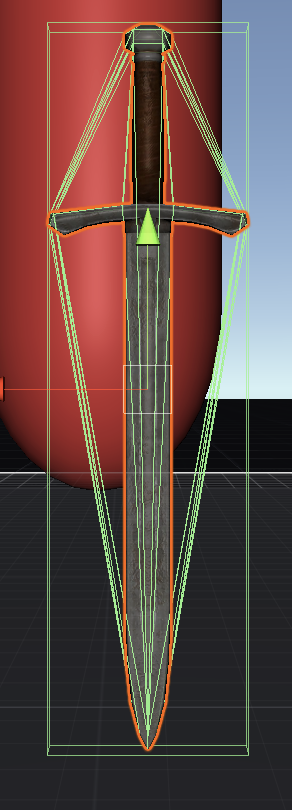
\includegraphics[width = 3cm ]{Sword_Colliders_Scene.png}}
        \caption{Box and Mesh collider in scene.}
    \end{minipage}
    \begin{minipage}{.8\textwidth}
        \centering
        \fbox{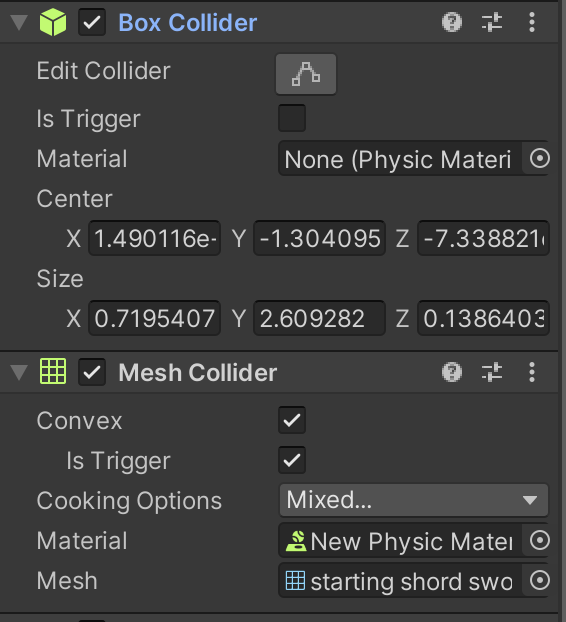
\includegraphics[width = 7cm ]{Sword_Colliders_Inspector.png}}
        \caption{Box and Mesh Colliders in the inspector.}
    \end{minipage}
\end{figure}

When the sword is in a state of attack, there is check in this collision whether it has collided with a game object with a life layer, and apply the damage value to the Stats component that exists on every creature.

\begin{lstlisting}[language=c]
// on Trigger Enter method, other is a parameter of type Collider
other.gameObject.GetComponent<Stats.Stats>().ApplyDamage(attackDamage, other.bounds.center, other.transform.rotation);

// Apply damage method in Stats.cs
public void ApplyDamage(float damage, Vector3 centerPosition, Quaternion rotation) {
    health -= damage;
    SpawnBloodParticles(centerPosition, rotation);
}

// spawning the particles on hit
public void SpawnBloodParticles(Vector3 centerPosition, Quaternion rotation) {
    Instantiate(bloodParticle, centerPosition, rotation);
}
\end{lstlisting}

% Crossbow
The ranged weapon was decided on being a crossbow that the player can hold right click to charge up the velocity at which it is release. A model was found on Turbosquid (see asset listing). This was imported into blender, and the crossbow and arrow were separated into two different objects, allowing it to be manipulated separately in Unity. A decision was made to not animate the crossbow as it is not crucial for the main aspect of this game.

This crossbow and arrow model were placed inside an empty called \textbf{RightHand} together and placed in the apropriate position in front of the player. An \textbf{arrow} prefab was created that contained the model of the arrow, a box collider, and a script attached to it to \textbf{ApplyDamage} on collision with an enemy creature similar to the sword. A script component was attached to the \textbf{RightHand} that instantiates an \textbf{arrow} prefab and give it a velocity. This was then adjusted to increase the velocity the longer the player holds down right-click up until a maximum velocity, and on release of the mouse button, the arrow gets released from the center of the camera view forwards. A GUI element was added to screen space canvas which represents the velocity at which the arrow will be released.
\begin{figure}[H]
    \begin{minipage}{.4\textwidth}
        \centering
        \fbox{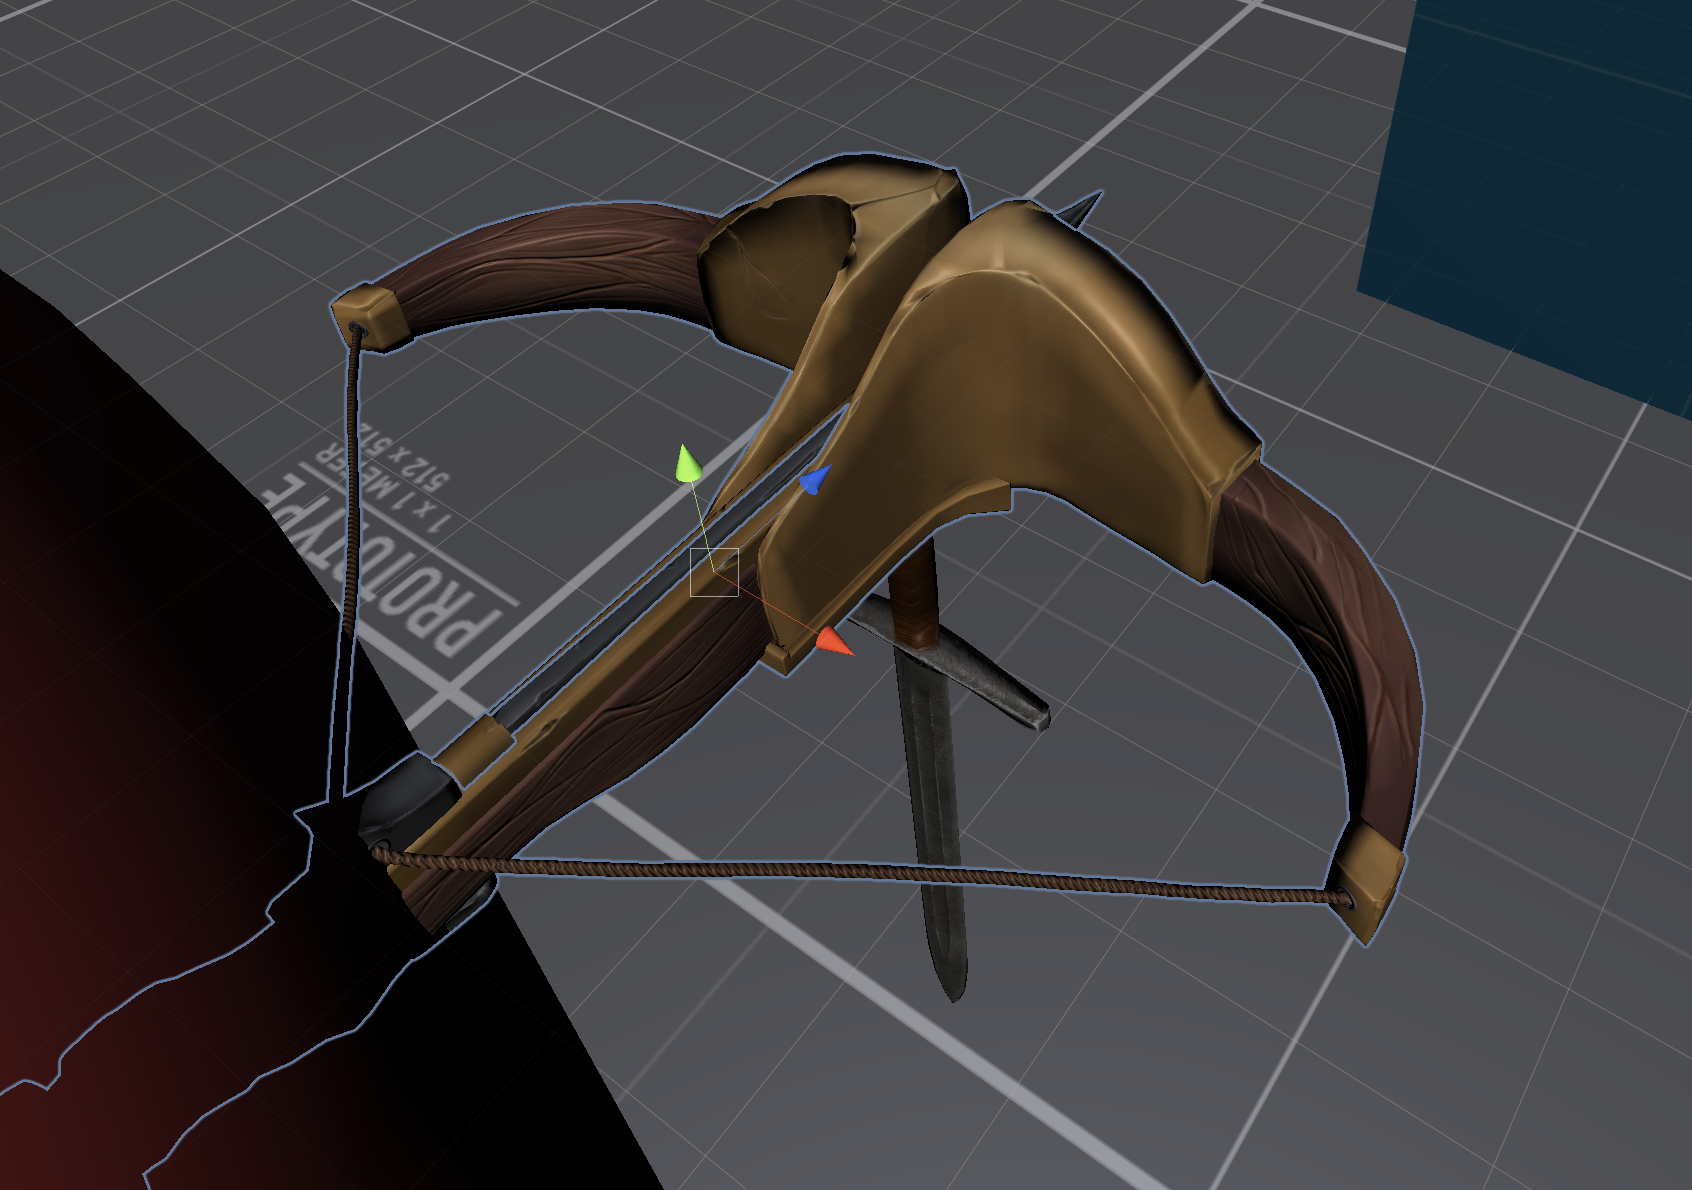
\includegraphics[width = 7cm ]{CrossBow_Scene.png}}
        \caption{Crossbow and arrow in the scene view}
    \end{minipage}
    \begin{minipage}{.6\textwidth}
        \centering
        \fbox{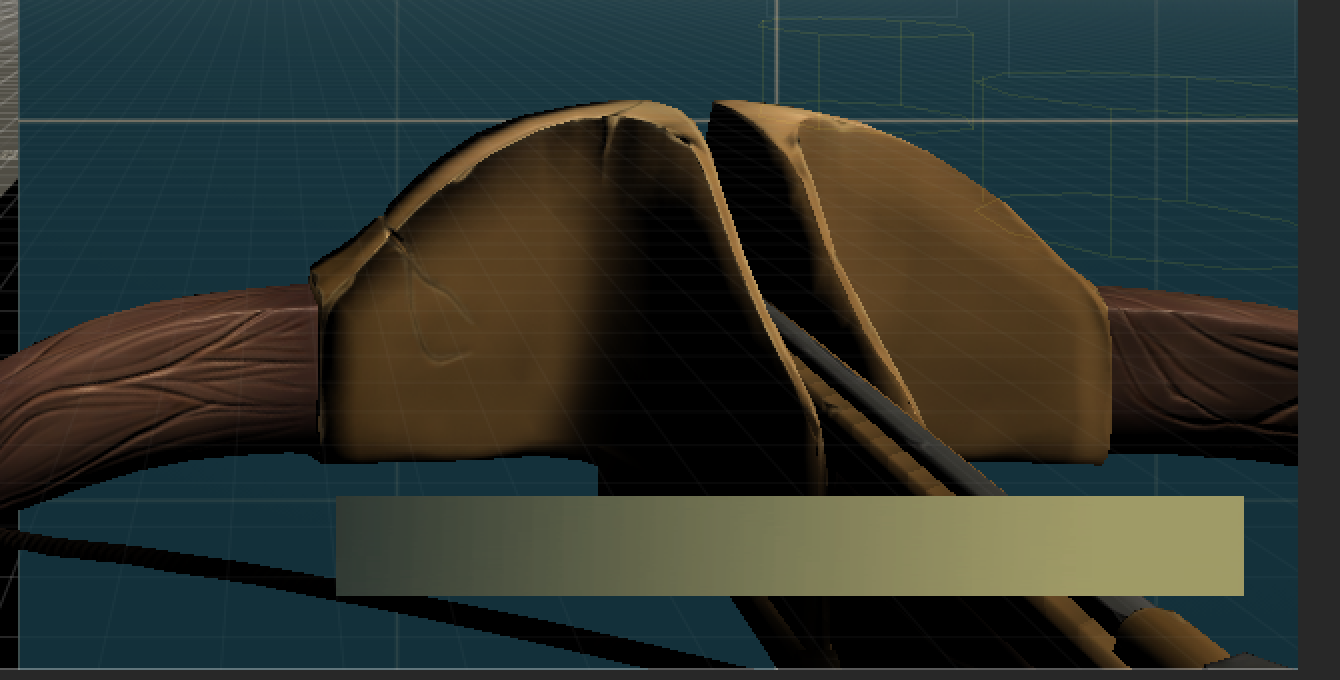
\includegraphics[width = 7cm ]{CrossBow_Game_With_GUI.png}}
        \caption{Crossbow in game view with GUI}
    \end{minipage}
\end{figure}

\subsection{Health}
When the PDD was created, the health was planned to be refilled using a collectible health resource which both the player and the creatures can pickup; however during development a better idea was formed. The health regeneration would be tied with the hunger, any excess food the agents or the player eats (excess being over 100) will refill the health for the creature/player. This encourages the player to interact with the game's core system of the food-chain and get into interesting gameplay for more food; an example of an interesting gameplay situation is the player observing that two predators are attacking each other, so to stay out of their vision cone range until they have depleted each-others health to a low amount and finish both 
off and eat the food.
This system is similar to that found in Minecraft \cite{minecraft}, where when the player's hunger is above/at max, the health will be regenerated.

\subsection{Stamina}
The stamina system that was created in build one of the 'Stats' component was being put into use now. The player swinging the sword would cost 15 points of stamina, and the regeneration rate is very slow at 2 points per second, with a total limit of 100. The player firing the crossbow would not cost any stamina; to add further distinction between the crossbow and sword, the sword does 50 damage per hit, potentially taking out an enemy in two hits, and the arrow does 10 damage per hit.

This allows for gameplay decisions that the player can make based on their situation, whether to get close, risk getting hurt, but taking the target/s out in 2 hits, \textit{or} stay at range, spend time aiming and charging the crossbow to fire a weaker shot, low risk, but lower damage hence taking longer to kill the target. The player can also run the risk of getting close, missing the sword swings and being out of stamina with only the crossbow to hit with. It is an interesting trade-off that the player will have to think about.

This was a successful implementation of a small aspect of the type of combat Dark Souls offers (as mentioned in the PDD, this is one of the inspirations for this project).

% creatures do not make use of the stamina

\subsection{Hunger}
The hunger for all creatures including the player depletes at a constant, albeit low rate; this simply simulates how in real life creatures get hungry over time, the different actions they have are directly tied into the level of hunger they are at, if they are below the threshold they will plan and perform actions to take that number above the threshold.

As mentioned before, the health is now tied into hunger, making it a necessity for the creatures to be above max huger to refill their health.

\subsection{User Interface changes}
The screen space UI/Heads up display was barren at this point, only including the charge bar for the crossbow.
As seen in the PDD and the introduction, the souls-like genre is an influence on this project, based on this, the Head was inspired from the games in that genre\cite{darkSouls3Wiki}.
\begin{figure}[H]
    \centering
    \fbox{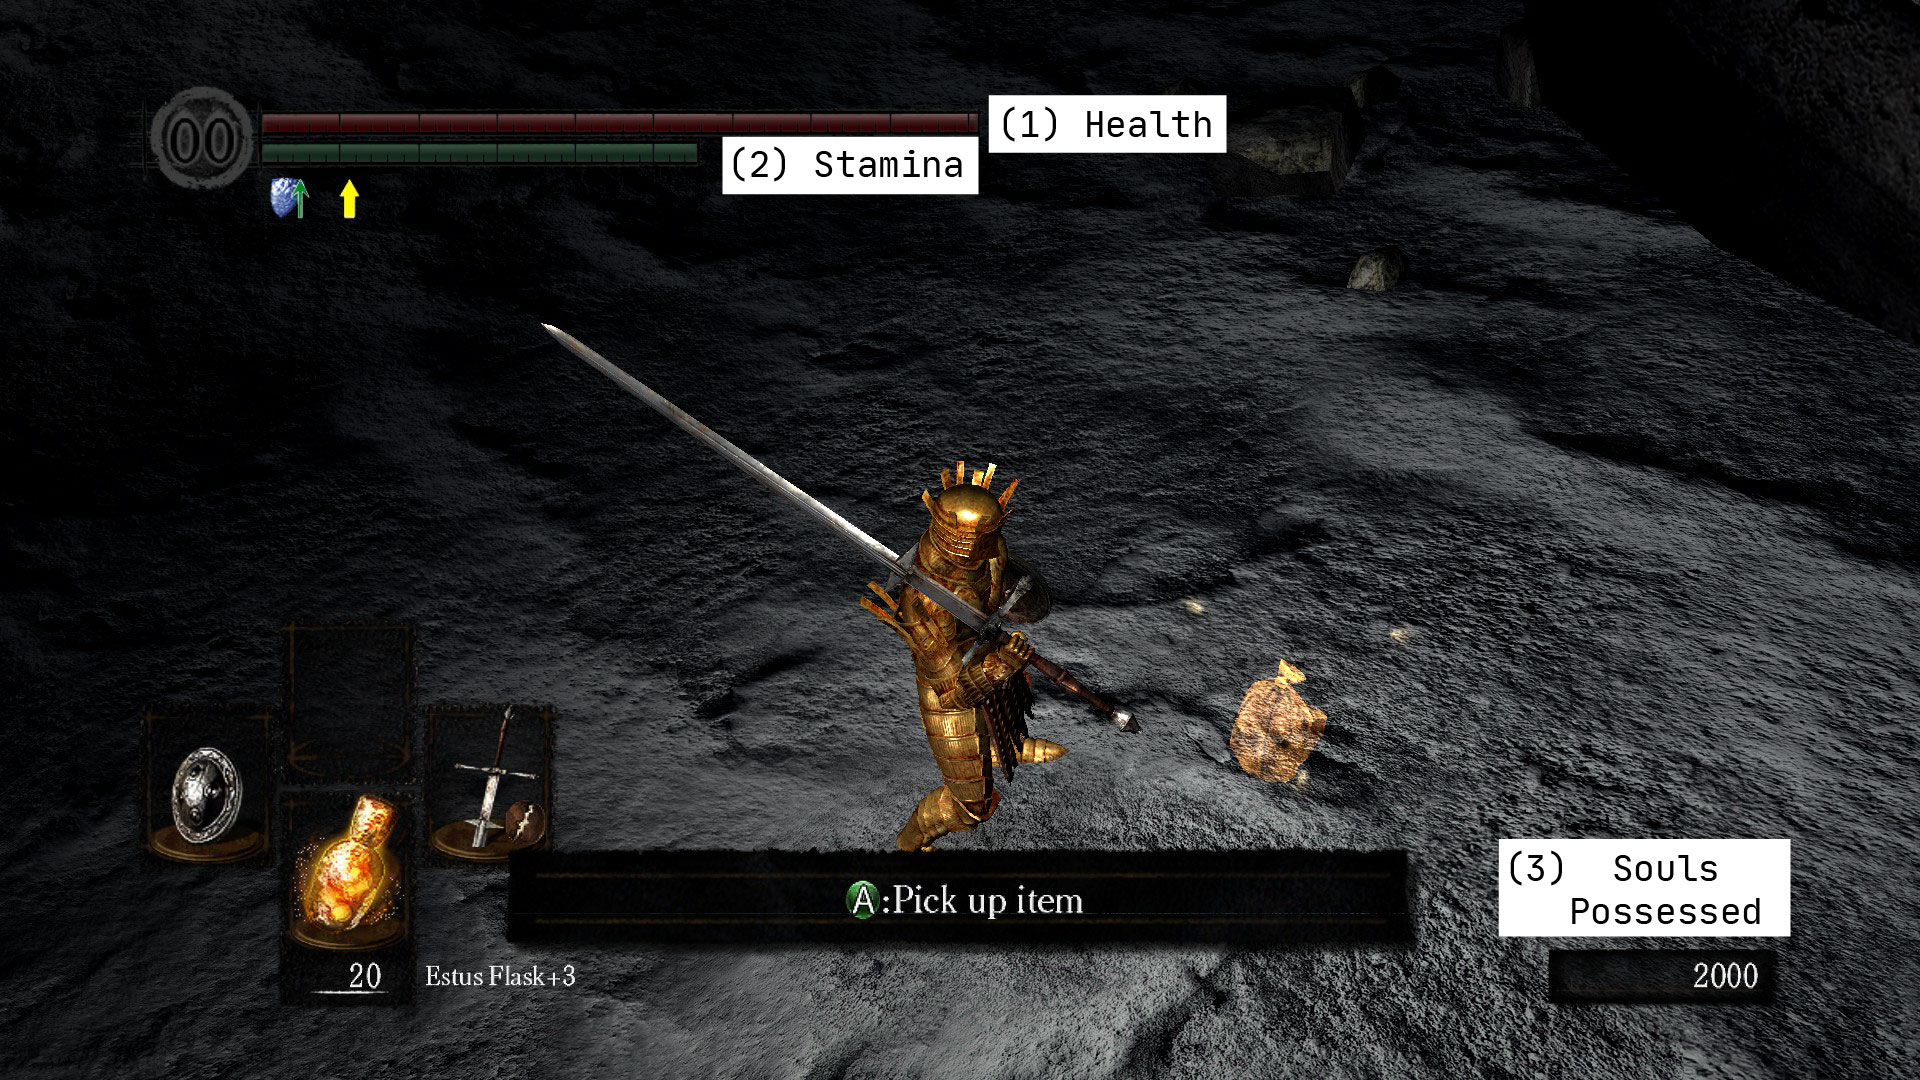
\includegraphics[width = 15cm]{darksouls3_hud_ui.jpg}}
    \caption{Heads up display in Dark Souls}
\end{figure}

The placement for the health(1) and stamina(2) were used for the health, hunger and stamina bar in this project. As there was no currency in this project, the Souls Possessed(3) positioning is replaced with the charge meter of the crossbow, leaving the bottom left and top right blank. 

In the figures below, you can see the sketch for the UI created in Adobe Illustrator and then the implementation of it inside of Unity. The indication to pick up items pops up in the center of the bottom of the screen, which in this project was moved out of the way adjacent the bars on the top left.
\begin{figure}[H]
    \centering
    \fbox{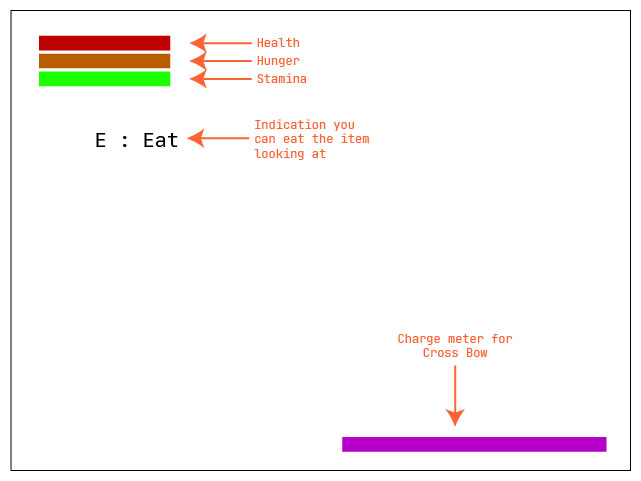
\includegraphics[width = 10cm]{Player_Hud_UI_Plan.jpg}}
    \caption{Sketch of Player HUD UI}
\end{figure}
\begin{figure}[H]
    \centering
    \fbox{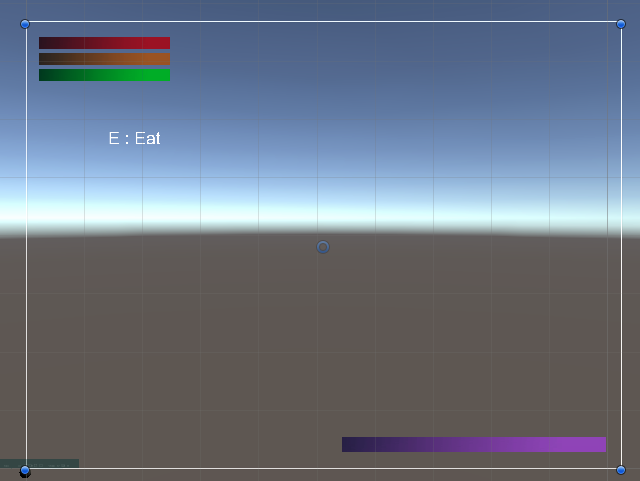
\includegraphics[width = 10cm]{Player_Hud_UI_Implementation.png}}
    \caption{Implementation of the Player's HUD in Unity.}
\end{figure}


\subsection{Level Creation}
As seen in the figure below, this was what the level where the different game systems were being tested looked like. After all the systems were created, a larger level was created to accommodate multiple enemies.
The main elements of the level was modeled in Blender, then unpacked with a texture applied in Unity; for the Pathfinding algorithm to detect these as obstacles, the “Obstacle” layer was applied to these objects. The stairs were built inside of Unity's ProBuilder, it has a tool to auto generate stairs with custom properties, like the curve added.
The creatures and plant were placed in random places, they all use the same prefab so changing the components in one, will change it in other instances of that game object.

For the objectives of this project, a win state is not necessary, there is however a death state for the player, when the player's life has been depleted, they will respawn, which is the scene is reloaded and the world state is reset to the beginning.

\begin{figure}[H]
    \begin{minipage}{.5\textwidth}
        \centering
        \fbox{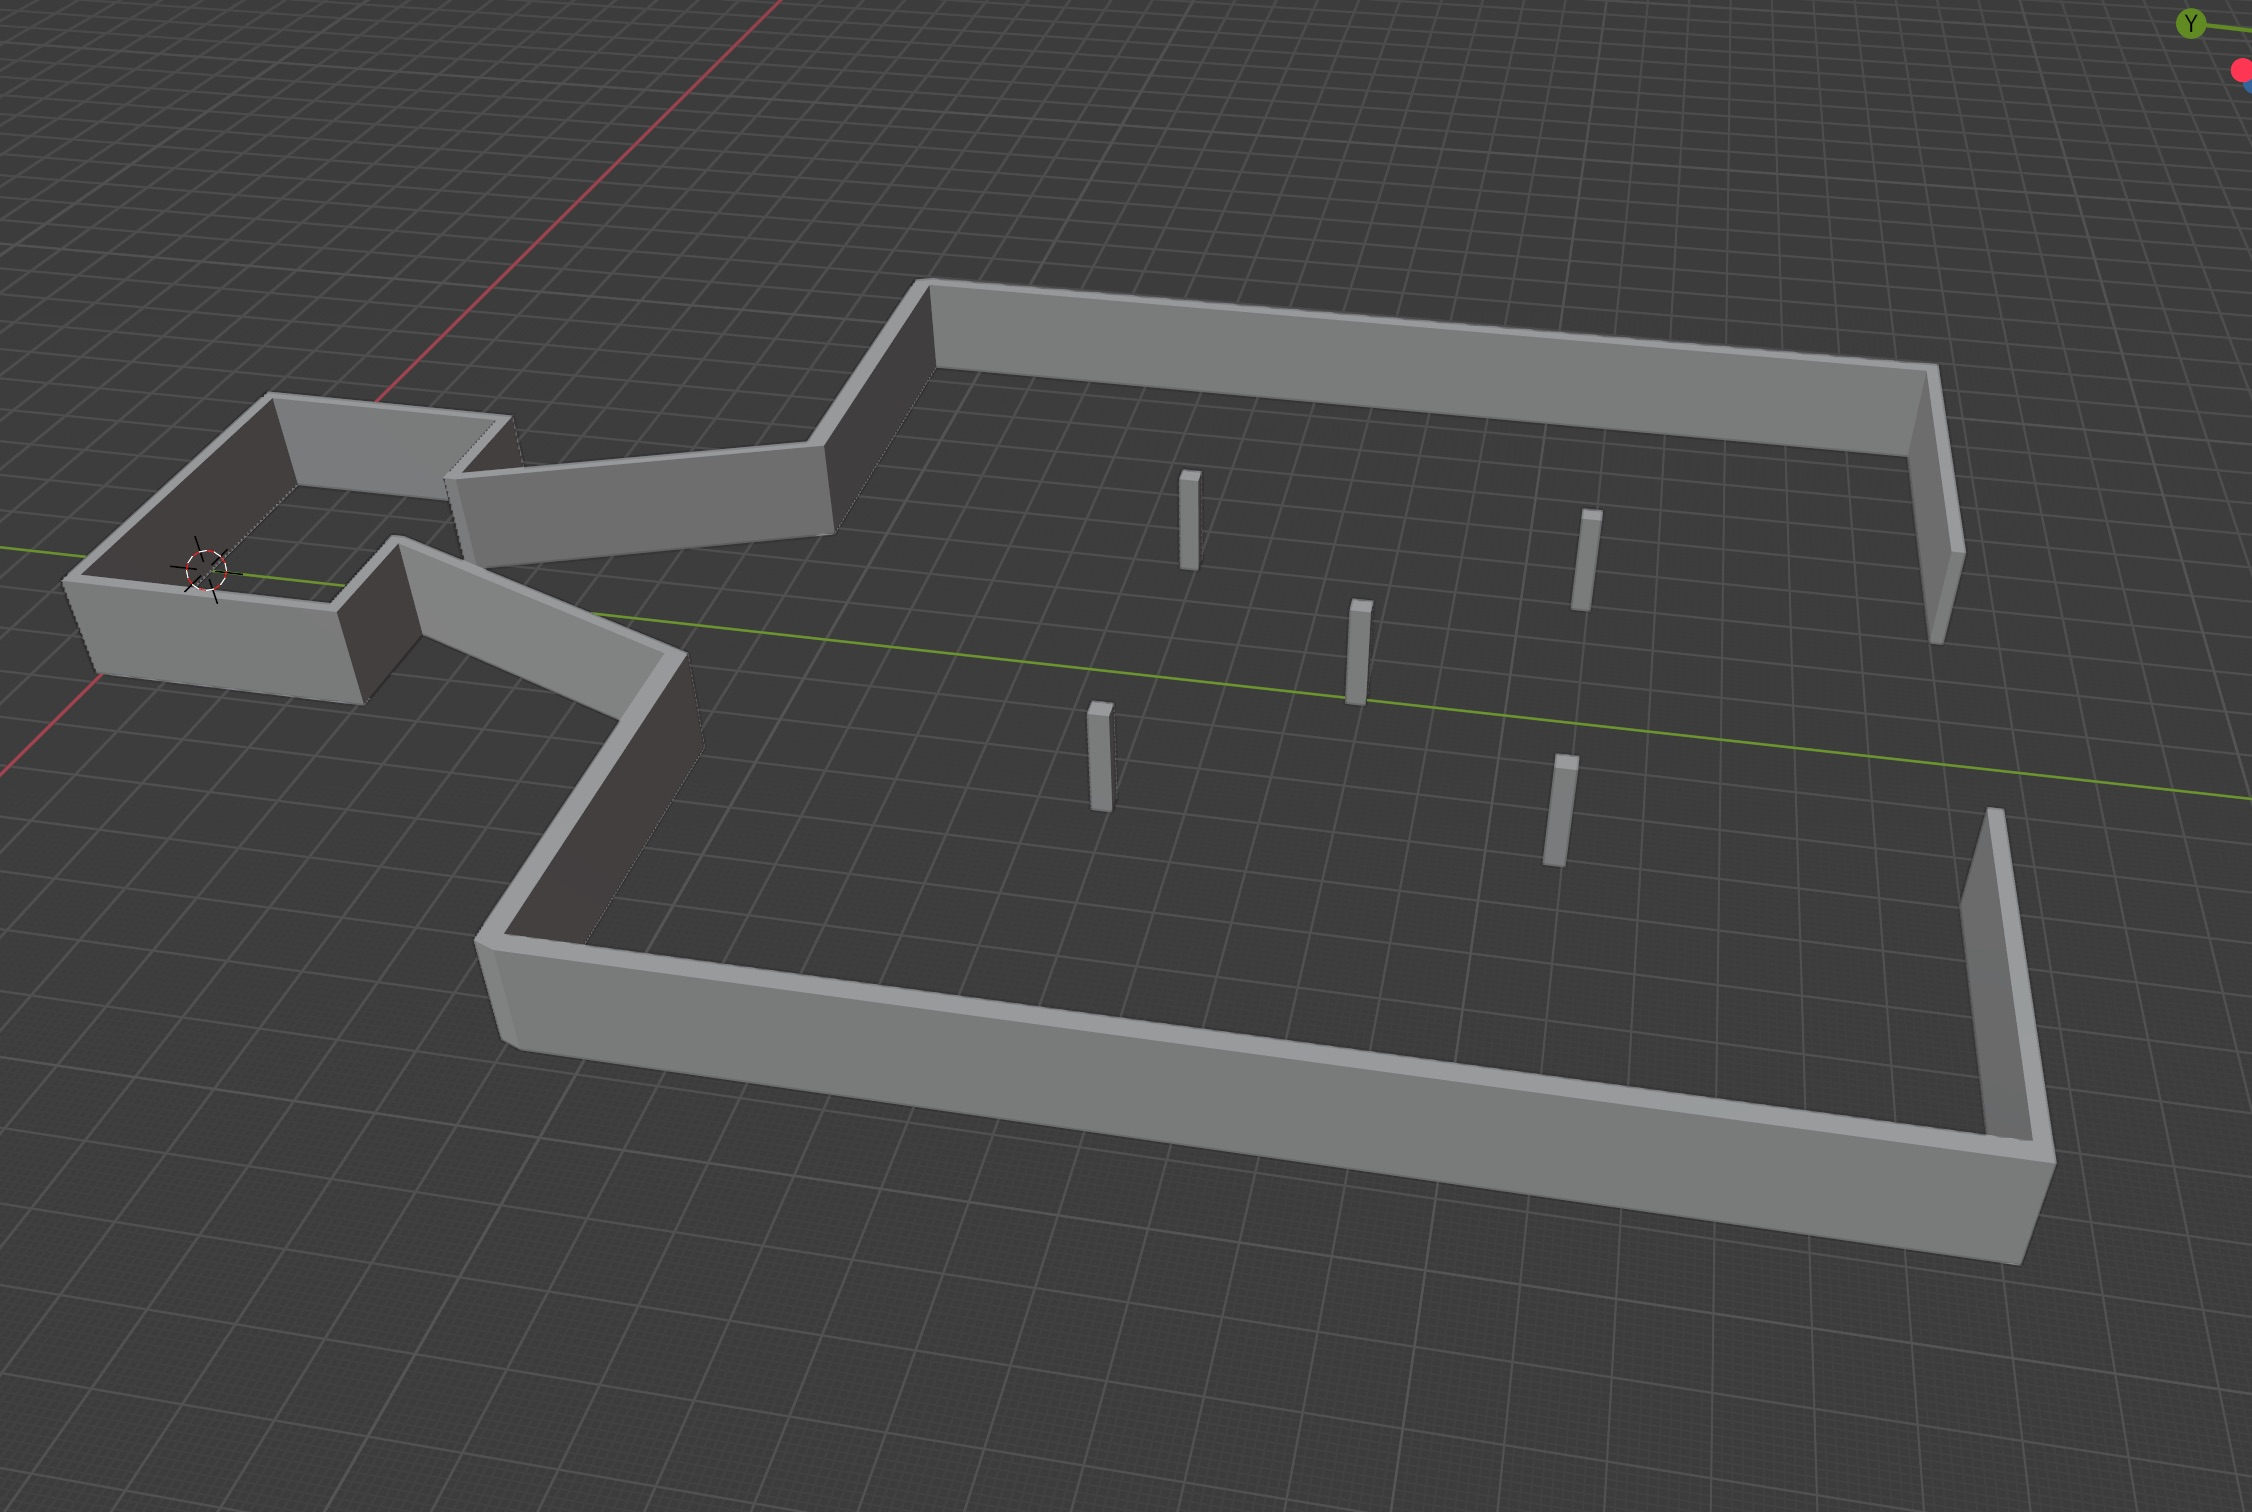
\includegraphics[width = 7cm ]{Level1_Blender.jpg}}
        \caption{Level Modelled inside of Blender}
    \end{minipage}
    \begin{minipage}{.5\textwidth}
        \centering
        \fbox{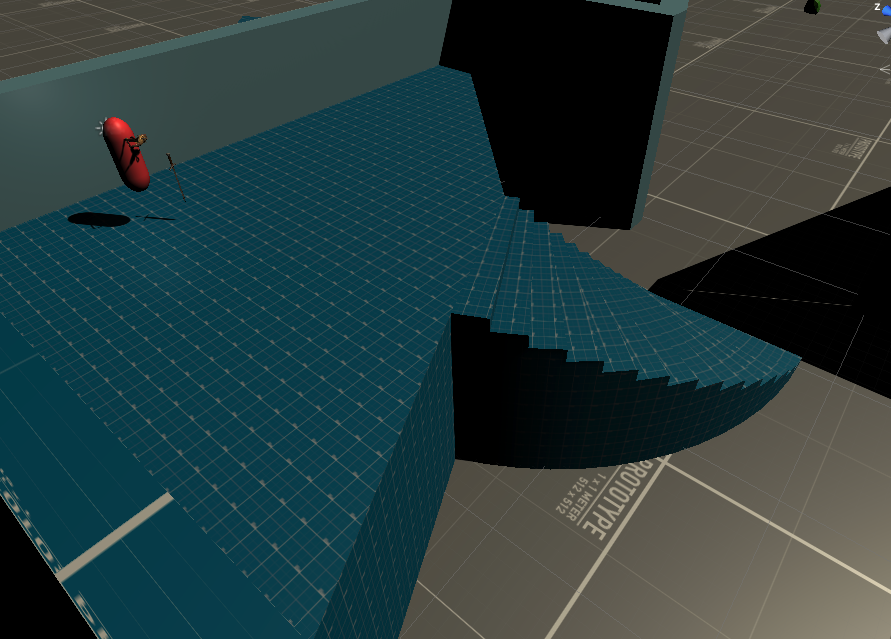
\includegraphics[width = 7cm ]{Level1_Stairs.png}}
        \caption{Stairs modelled in ProBuilder inside of Unity}
    \end{minipage}
\end{figure}

\begin{figure}[H]
    \centering
    \fbox{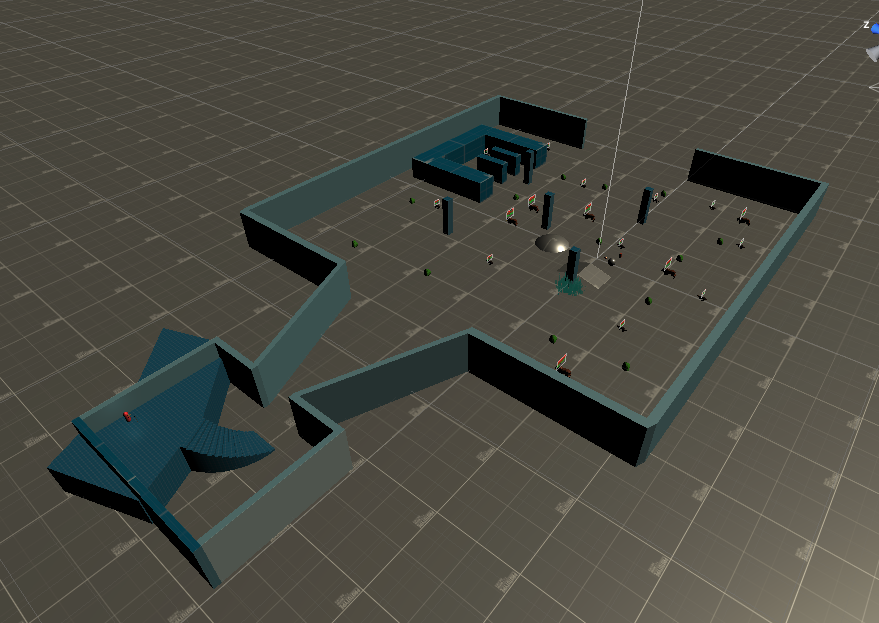
\includegraphics[width = 15cm]{Level1_Unity.png}}
    \caption{Level in Unity}
\end{figure}

%=========================
%   Asset Listings
%=========================
\chapter{Asset Listing}

%=========================
%   References / Bibliography
%=========================
\begin{thebibliography}{}
    \bibitem{doom93}
    id Software, id Software, (1993). DOOM. [computer game]. \\Available at: \url{https://store.bethesda.net/store/bethesda/en_IE/pd/productID.5361563100/currency.GBP}
    \bibitem{farcry}
    Ubisoft.com. 2021. Far Cry franchise. [online] Available at: \url{https://www.ubisoft.com/en-gb/franchise/far-cry/} [Accessed 9 February 2021].
    \bibitem{farCryPrimalCompanions}
    Thompson, T., 2018. Primal Instinct | Companion AI in Far Cry Primal. [online] Gamasutra.com. Available at: \url{https://gamasutra.com/blogs/TommyThompson/20180906/325967/Primal_Instinct__Companion_AI_in_Far_Cry_Primal.php} [Accessed 12 February 2021].
    \bibitem{emergentGameplay}
    "Le Gameplay emergent (in French)". jeuxvideo.com. 2006-01-19. Available at: \url{https://www.jeuxvideo.com/dossiers/00006203/le-gameplay-emergent.htm} [Accessed 9th February 2021]
    \bibitem{gameAiByExample}
    Buckland, M., 2010. Programming Game AI by Example. Burlington: Jones \& Bartlett Learning, LLC, p.46.
    \bibitem{halo2}
    Bungie, Microsoft Game Studios. Halo 2 [computer game]. 04/09/2004.
    \bibitem{behaviourTrees}
    Simpson, C., 2014. Behavior trees for AI: How they work. [online] Gamasutra.com. Available at: \url{https://www.gamasutra.com/blogs/ChrisSimpson/20140717/221339/Behavior_trees_for_AI_How_they_work.php} [Accessed 12 February 2021].
    \bibitem{goap}
    Orkin, J., n.d. Goal-Oriented Action Planning (GOAP). [online] \\Alumni.media.mit.edu. Available at: \url{http://alumni.media.mit.edu/~jorkin/goap.html} [Accessed 12 February 2021].
    \bibitem{applyingGoap}
    Orkin, J., n.d. Applying Goal-Oriented Action Planning to Games. [online] \\Alumni.media.mit.edu. Available at: \url{http://alumni.media.mit.edu/~jorkin/GOAP_draft_AIWisdom2_2003.pdf} [Accessed 12 February 2021].
    \bibitem{goapTommyTompson}
    Thompson, T., 2020. Building the AI of F.E.A.R. with Goal Oriented Action Planning. [online] Gamasutra.com. Available at: \url{https://www.gamasutra.com/blogs/TommyThompson/20200507/362417/Building_the_AI_of_FEAR_with_Goal_Oriented_Action_Planning.php} [Accessed 13 February 2021].
    \bibitem{fearSDK}
    Monolith Productions, Inc., 2004, Fear SDK 1.08 [code] Available at: \url{http://fear.filefront.com/file/FEAR_v108_SDK;71433} and \url{https://github.com/xfw5/Fear-SDK-1.08.git}
    \bibitem{basherGoap}
    Klooster, Peter, GOAP, a multi-threaded library for Unity [code] Available at: \url{https://github.com/crashkonijn/GOAP}, under Apache-2.0 licence
    \bibitem{happieGoapVideo}
    Anne, 2016. Combat AI for Action-Adventure Games Tutorial [Unity/C\#] [GOAP]. [video] Available at: \url{https://youtu.be/n6vn7d5R_2c} [Accessed 13 February 2021].
    \bibitem{brentOwensGoap}
    Owens, B., 2014. Goal Oriented Action Planning for a Smarter AI. [online] Game Development Envato Tuts+. Available at: \url{https://gamedevelopment.tutsplus.com/tutorials/goal-oriented-action-planning-for-a-smarter-ai--cms-20793} [Accessed 13 February 2021].
    \bibitem{brentOwensGoapCode}
    Owens, B., 2014. Goal Oriented Action Planning for a Smarter AI. [code]. Available at: \url{https://github.com/sploreg/goap} [Accessed 13 February 2021].
    \bibitem{drawIo}
    App.diagrams.net. 2021. Flowchart Maker \& Online Diagram Software. [online] Available at: \url{https://app.diagrams.net/} [Accessed 20 February 2021].
    \bibitem{codingPractices}
    En.wikipedia.org. n.d. Coding best practices - Wikipedia. [online] Available at: \url{https://en.wikipedia.org/wiki/Coding_best_practices} [Accessed 15 April 2021].
    \bibitem{CompOverInherit}
    Youtu.be. 2021. Composition over Inheritance. [online] Available at: \url{https://youtu.be/wfMtDGfHWpA} [Accessed 15 April 2021].
    \bibitem{UIChoices}
    F, J., 2021. What Are Your UI Choices. [online] Medium. Available at: \url{https://medium.com/@gfruity/what-are-your-ui-choices-834ea7d937c} [Accessed 18 April 2021].
    \bibitem{comboSystem}
    Grimoirehex.com. 2017. Unity 3D – Combo System Animation – GRIMOIRE. [online] Available at: \url{https://www.grimoirehex.com/unity-3d-combo-animation/} [Accessed 15 February 2021].
    \bibitem{astarPathfinding}
    Granberg, A., 2017. Documentation. [online] Arongranberg.com. Available at: \url{https://arongranberg.com/astar/docs/graphtypes.html} [Accessed 20 April 2021].
    \bibitem{UnityTriggerCollider}
    Technologies, U., 2021. Unity - Scripting API: Collider.OnTriggerEnter(Collider). [online] Docs.unity3d.com. Available at: \url{https://docs.unity3d.com/ScriptReference/Collider.OnTriggerEnter.html} [Accessed 20 April 2021].
    \bibitem{AgileMethodology}
    UKEssays.com. 2021. Rapid Application Development vs. Agile Methodologies. [online] Available at: \url{https://www.ukessays.com/essays/management/rapid-application-development-vs-agile-methodologies.php} [Accessed 21 February 2021].
    \bibitem{RagdollTutorial}
    DitzelGames, 2021. Create an Animal Ragdoll in Unity. [image] Available at: \url{https://youtu.be/oVPI2ESkgIw} [Accessed 1 April 2021].
    \bibitem{darkSouls3Wiki}
    Fextralife, 2021. Dark Souls 3. [online] Dark Souls 3 Wiki. Available at: \url{https://darksouls3.wiki.fextralife.com/Dark+Souls+3} [Accessed 15 April 2021]. 
    \bibitem{fpsController}
    Brackeys. 2021. FIRST PERSON MOVEMENT in Unity - FPS Controller. [online] Available at: \url{https://www.youtube.com/watch?v=_QajrabyTJc} [Accessed 5 February 2021].
    \bibitem{biDirectionalDictionaries}
    erdiizgi.com. n.d. Data Structures for Games: Bidirectional Dictionary for Unity in C\#. [online] Available at: \url{https://erdiizgi.com/data-structures-for-games-bidirectional-dictionary-for-unity-in-c/} [Accessed 26 April 2021].
    \bibitem{minecraft}
    Minecraft. 2021. [computer game] \url{https://www.minecraft.net/en-us/}: Mojang, Microsoft.
    \bibitem{godot}
    2021. Godot Game Engine v3.3. \url{https://godotengine.org/}: Godot.
    \bibitem{unrealEngine}
    2021. Unreal Engine 4. \url{https://www.unrealengine.com}: Epic Games.
    \bibitem{unity}
    2021. Unity Game Engine. \url{https://unity.com/}: Unity Technologies.
\end{thebibliography}
\end{document}